\chapter{Sprint 1 : Enhancements and Integrations}

\section{Introduction}
In this chapter, we cover the first sprint of the Aermax project, focusing on the key enhancements and features we implemented to improve the platform.
\setcounter{secnumdepth}{0}
\section{Major Features and Enhancements}

\subsection{Sprint Backlog Detail}
Below is a detailed representation of our sprint backlog, showcasing the major tasks we committed to delivering in Sprint 1. We fixed around \textbf{26+ bugs, feature enhancements,} and new features in Sprint 1. Below, we're going to share some of them.

% Set up the longtable environment to break across pages
\begin{longtable}{|p{2.5cm}|p{2cm}|p{2.75cm}|p{1.75cm}|p{1.75cm}|p{1.25cm}|}

    % Table header information
    \caption{Detailed Sprint Backlog} \\
    \hline
    \textbf{Type} & \textbf{Title} & \textbf{Description} & \textbf{Priority} & \textbf{Assignee} & \textbf{Status} \\
    \hline
    \endfirsthead
    
    % Table continuation header information
    \multicolumn{6}{c}%
    {{\bfseries Table \thetable\ Continued from previous page}} \\
    \hline
    \textbf{Type} & \textbf{Title} & \textbf{Description} & \textbf{Priority} & \textbf{Assignee} & \textbf{Status} \\
    \hline
    \endhead
    
    % Footer at the end of each page (if needed)
    \hline
    \multicolumn{6}{|r|}{{Continued on next page}} \\ \hline
    \endfoot
    
    % Footer at the end of the table (if needed)
    \hline
    \endlastfoot
    
    % Table content
    Feature & Implement Self-Registration & Allow subcontractors to self-register on the platform. & High & Donia Skima & Done \\    \hline
    Enhancement & Adjust Feedback Notification & Update feedback functionality to include notifications in teams. & Medium & Ramez Taher & Done \\
    \hline
    Enhancement & Set Dynamic Project Status & Dynamically set project status based on packet statuses. & High & Donia Skima & Done \\
    \hline
    Enhancement & Add Field to User Edit & Include additional fields in the user edit form. & Medium & Donia Skima & Done \\
    \hline
    Feature & Set Default Calendar View & Remember last selection for default calendar view using localStorage. & Medium & Ramez Taher & Done \\
    \hline
    Enhancement & Restrict Project Creation & Prevent subcontractors from creating new projects. & High & Ramez Taher & Done \\
    \hline
    Enhancement & Remove Team Types & Remove unnecessary team types from the app to streamline functionality. & Low & Donia Skima & Done \\
    \hline
    Feature & Calendar View with New Filters & Implement new filters for the calendar view for better UX. & High & Ramez Taher & Done \\
    \hline
    Feature & Implement Google Maps URL Generation & Generate Google Maps URLs for address visualization in subcompany user view. & Medium & Donia Skima & Done \\
    \hline
    Bug & Overhaul User Access Restrictions & Fix critical access restrictions and bugs for subcompany users. & High & Donia Skima & Done \\
    \hline
    Feature & Overhaul the Role System & Revise the role system to clarify permissions and responsibilities. & High & Donia Skima & Done \\
    \hline
    Feature & Automate Username Generation & Auto-generate usernames during self-registration. & Medium & Donia Skima & Done \\
    \hline
    Feature & Remember Date Filters for Calendar & Implement a feature to remember date filters for the calendar. & Low & Ramez Taher & Done \\
    \hline
    Feature & Overhaul the Project Status & Update project status features and adjust status enums and filters. & High & Ramez Taher & Done \\
    \hline
    Bug & Fix Read-Only State of User Edit Form & Correct the issue with the user edit form being read-only for admins. & Medium & Donia Skima & Done \\
    \hline
    Bug & Remove Duplicate Aggregated Phases & Remove any duplicate instances of aggregated phases in the system. & High & Donia Skima & Done \\
    \hline
    Enhancement & Enhance Working Packets UI \& UX & Improve the UI and UX for working packets. & Medium & Ramez Taher & Done \\
    \hline
    Feature & Dynamic Equipment List & The ticket describes an issue with a dynamic equipment list system where equipment items are grouped and managed. & High & Donia Skima & Done \\
    \hline
    \end{longtable}
    \subsection{Dynamic Equipment List}
    \subsubsection{Dynamic Equipment List issues}
    The Dynamic Equipment List feature was previously implemented as a static list. This static list required manual updates and did not reflect real-time changes to the equipment database. The key characteristics of the static implementation included:
    \begin{itemize}
        \item Manual updates to the equipment list.
        \item Limited flexibility and responsiveness to changes.
        \item High maintenance overhead due to frequent updates.
    \end{itemize}
    
    \subsubsection{Issues with Static Implementation}
    The static implementation had several drawbacks:
    \begin{itemize}
        \item \textbf{Scalability:} As the number of equipment items grew, maintaining the static list became increasingly cumbersome.
        \item \textbf{Real-time Updates:} Any changes to the equipment database were not immediately reflected in the list, leading to potential inconsistencies.
        \item \textbf{User Experience:} Users could not rely on the list for up-to-date information, which impacted their ability to make informed decisions.
    \end{itemize}
    
    \begin{figure}[H]
        \centering
        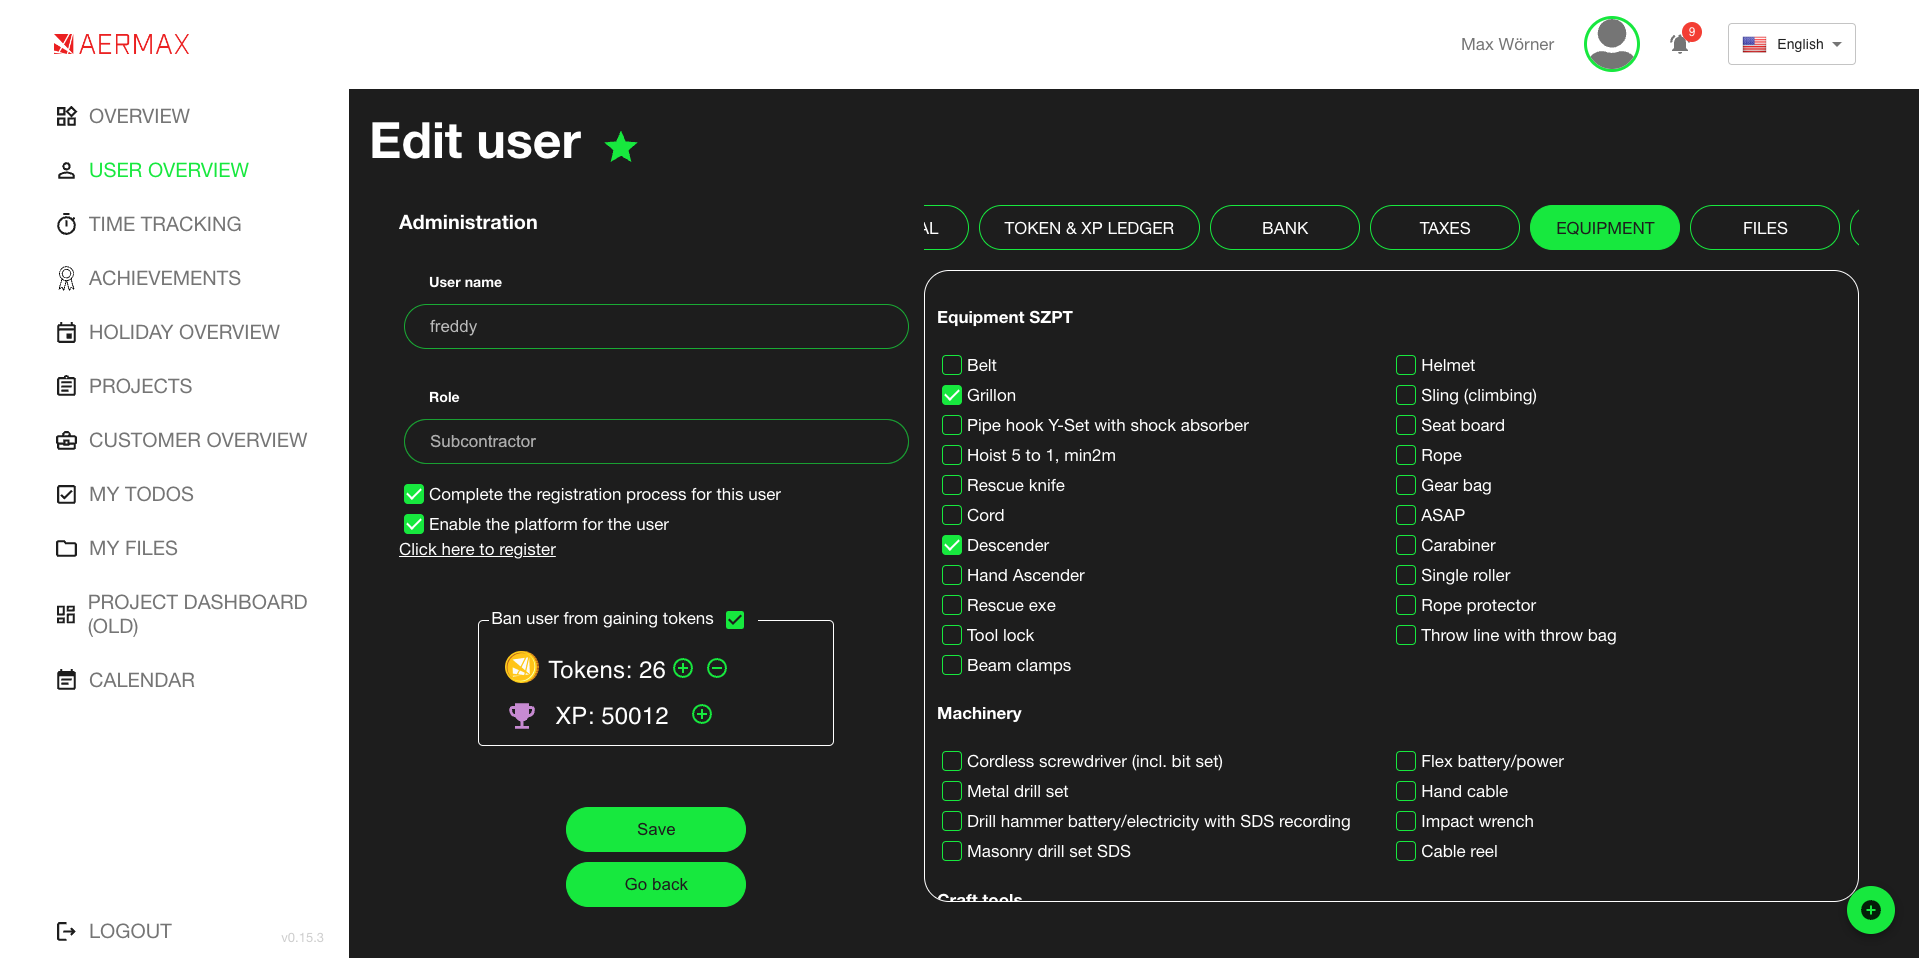
\includegraphics[width=0.9\textwidth]{src/assets/chapters/StaticDynamicEquipementList.png}
        \caption{Previous Static Equipment List}
        \label{fig:static_equipment_list}
    \end{figure}
    
    \subsubsection{Dynamic Equipment List Solution}
    To address these issues, we are transitioning to a dynamic equipment list. The dynamic implementation will automatically update the list based on changes in the equipment database, ensuring real-time accuracy and reducing maintenance overhead. Key features of the dynamic implementation include:
    \begin{itemize}
        \item \textbf{Real-time Updates:} The list will automatically reflect changes made to the equipment database.
        \item \textbf{Improved Scalability:} The system can handle an increased number of equipment items without additional maintenance.
        \item \textbf{Request System:} Subcontractors can request new equipment, and the admin can approve or reject these requests.
        \item \textbf{Reduced Maintenance:} Eliminates the need for manual updates, reducing the time and effort required to maintain the list.
    \end{itemize}
    
    The diagram below illustrates the planned dynamic equipment list from the admin's perspective (see Fig. \ref{fig:dynamic_equipment_list_admin}).

    \begin{figure}[H]
        \centering
        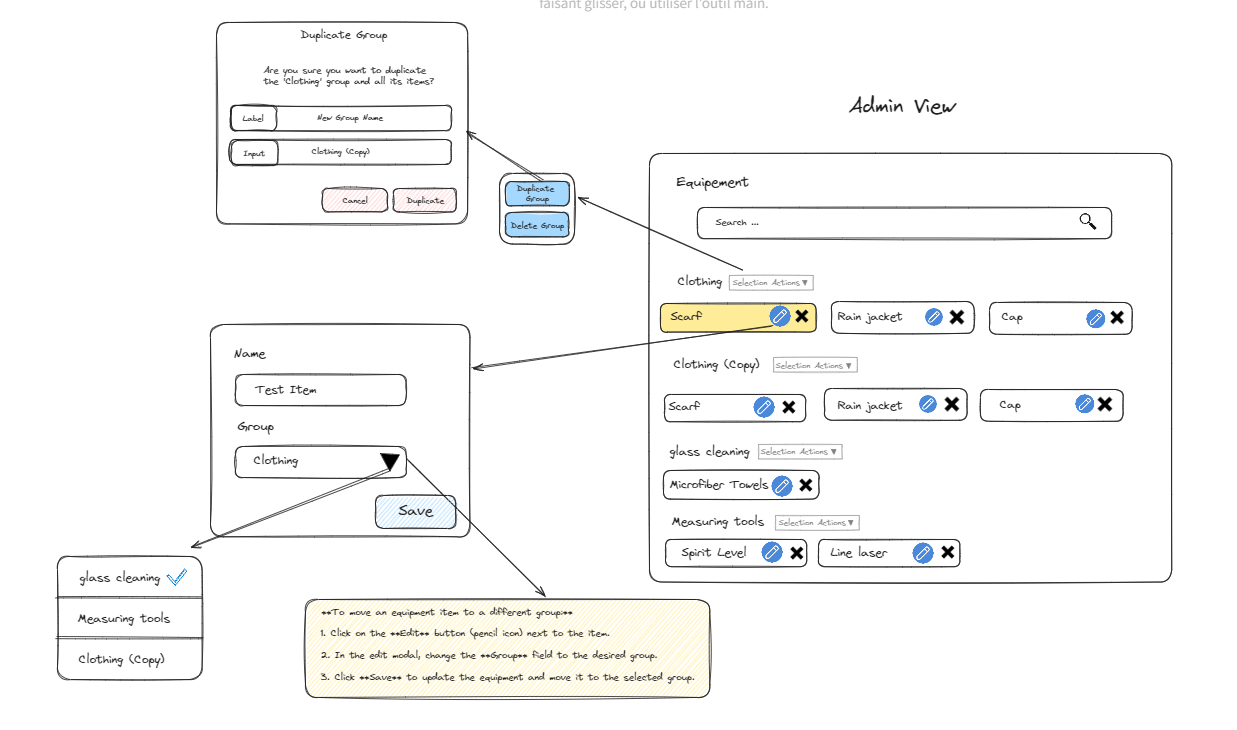
\includegraphics[width=0.9\textwidth]{src/assets/chapters/DynamicEquipementAdmin.PNG}
        \caption{Planned Dynamic Equipment List - Admin View}
        \label{fig:dynamic_equipment_list_admin}
    \end{figure}
    
    \begin{figure}[H]
        \centering
        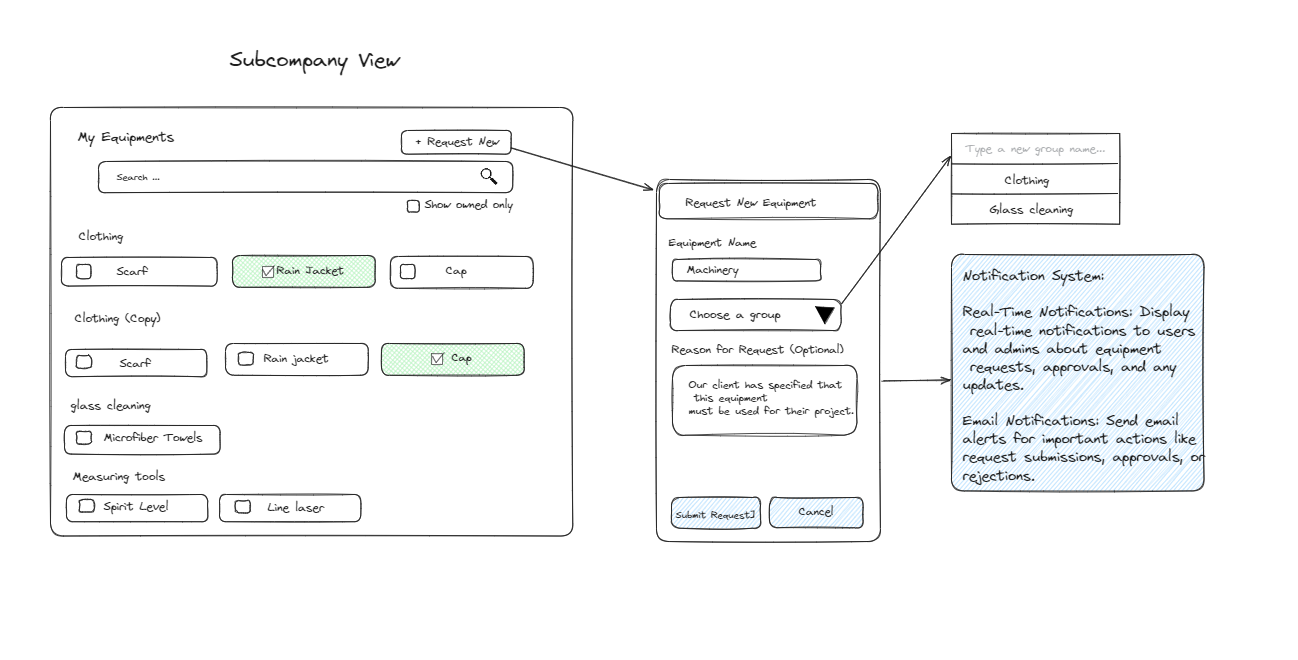
\includegraphics[width=0.9\textwidth]{src/assets/chapters/DynamicEquipementSubcompany.PNG}
        \caption{Planned Dynamic Equipment List - Subcompany View}
        \label{fig:dynamic_equipment_list_subcompany}
    \end{figure}
    \subsubsection{Dynamic Equipment Design}
To effectively transition from a static to a dynamic equipment list, we need to carefully design the system architecture. The following sections provide a detailed overview of the class structure and interactions.

\paragraph{Class Diagram}
The class diagram below illustrates the key components and relationships involved in the dynamic equipment list feature (see Fig. \ref{fig:class_diagram}).

\begin{figure}[H]
    \centering
    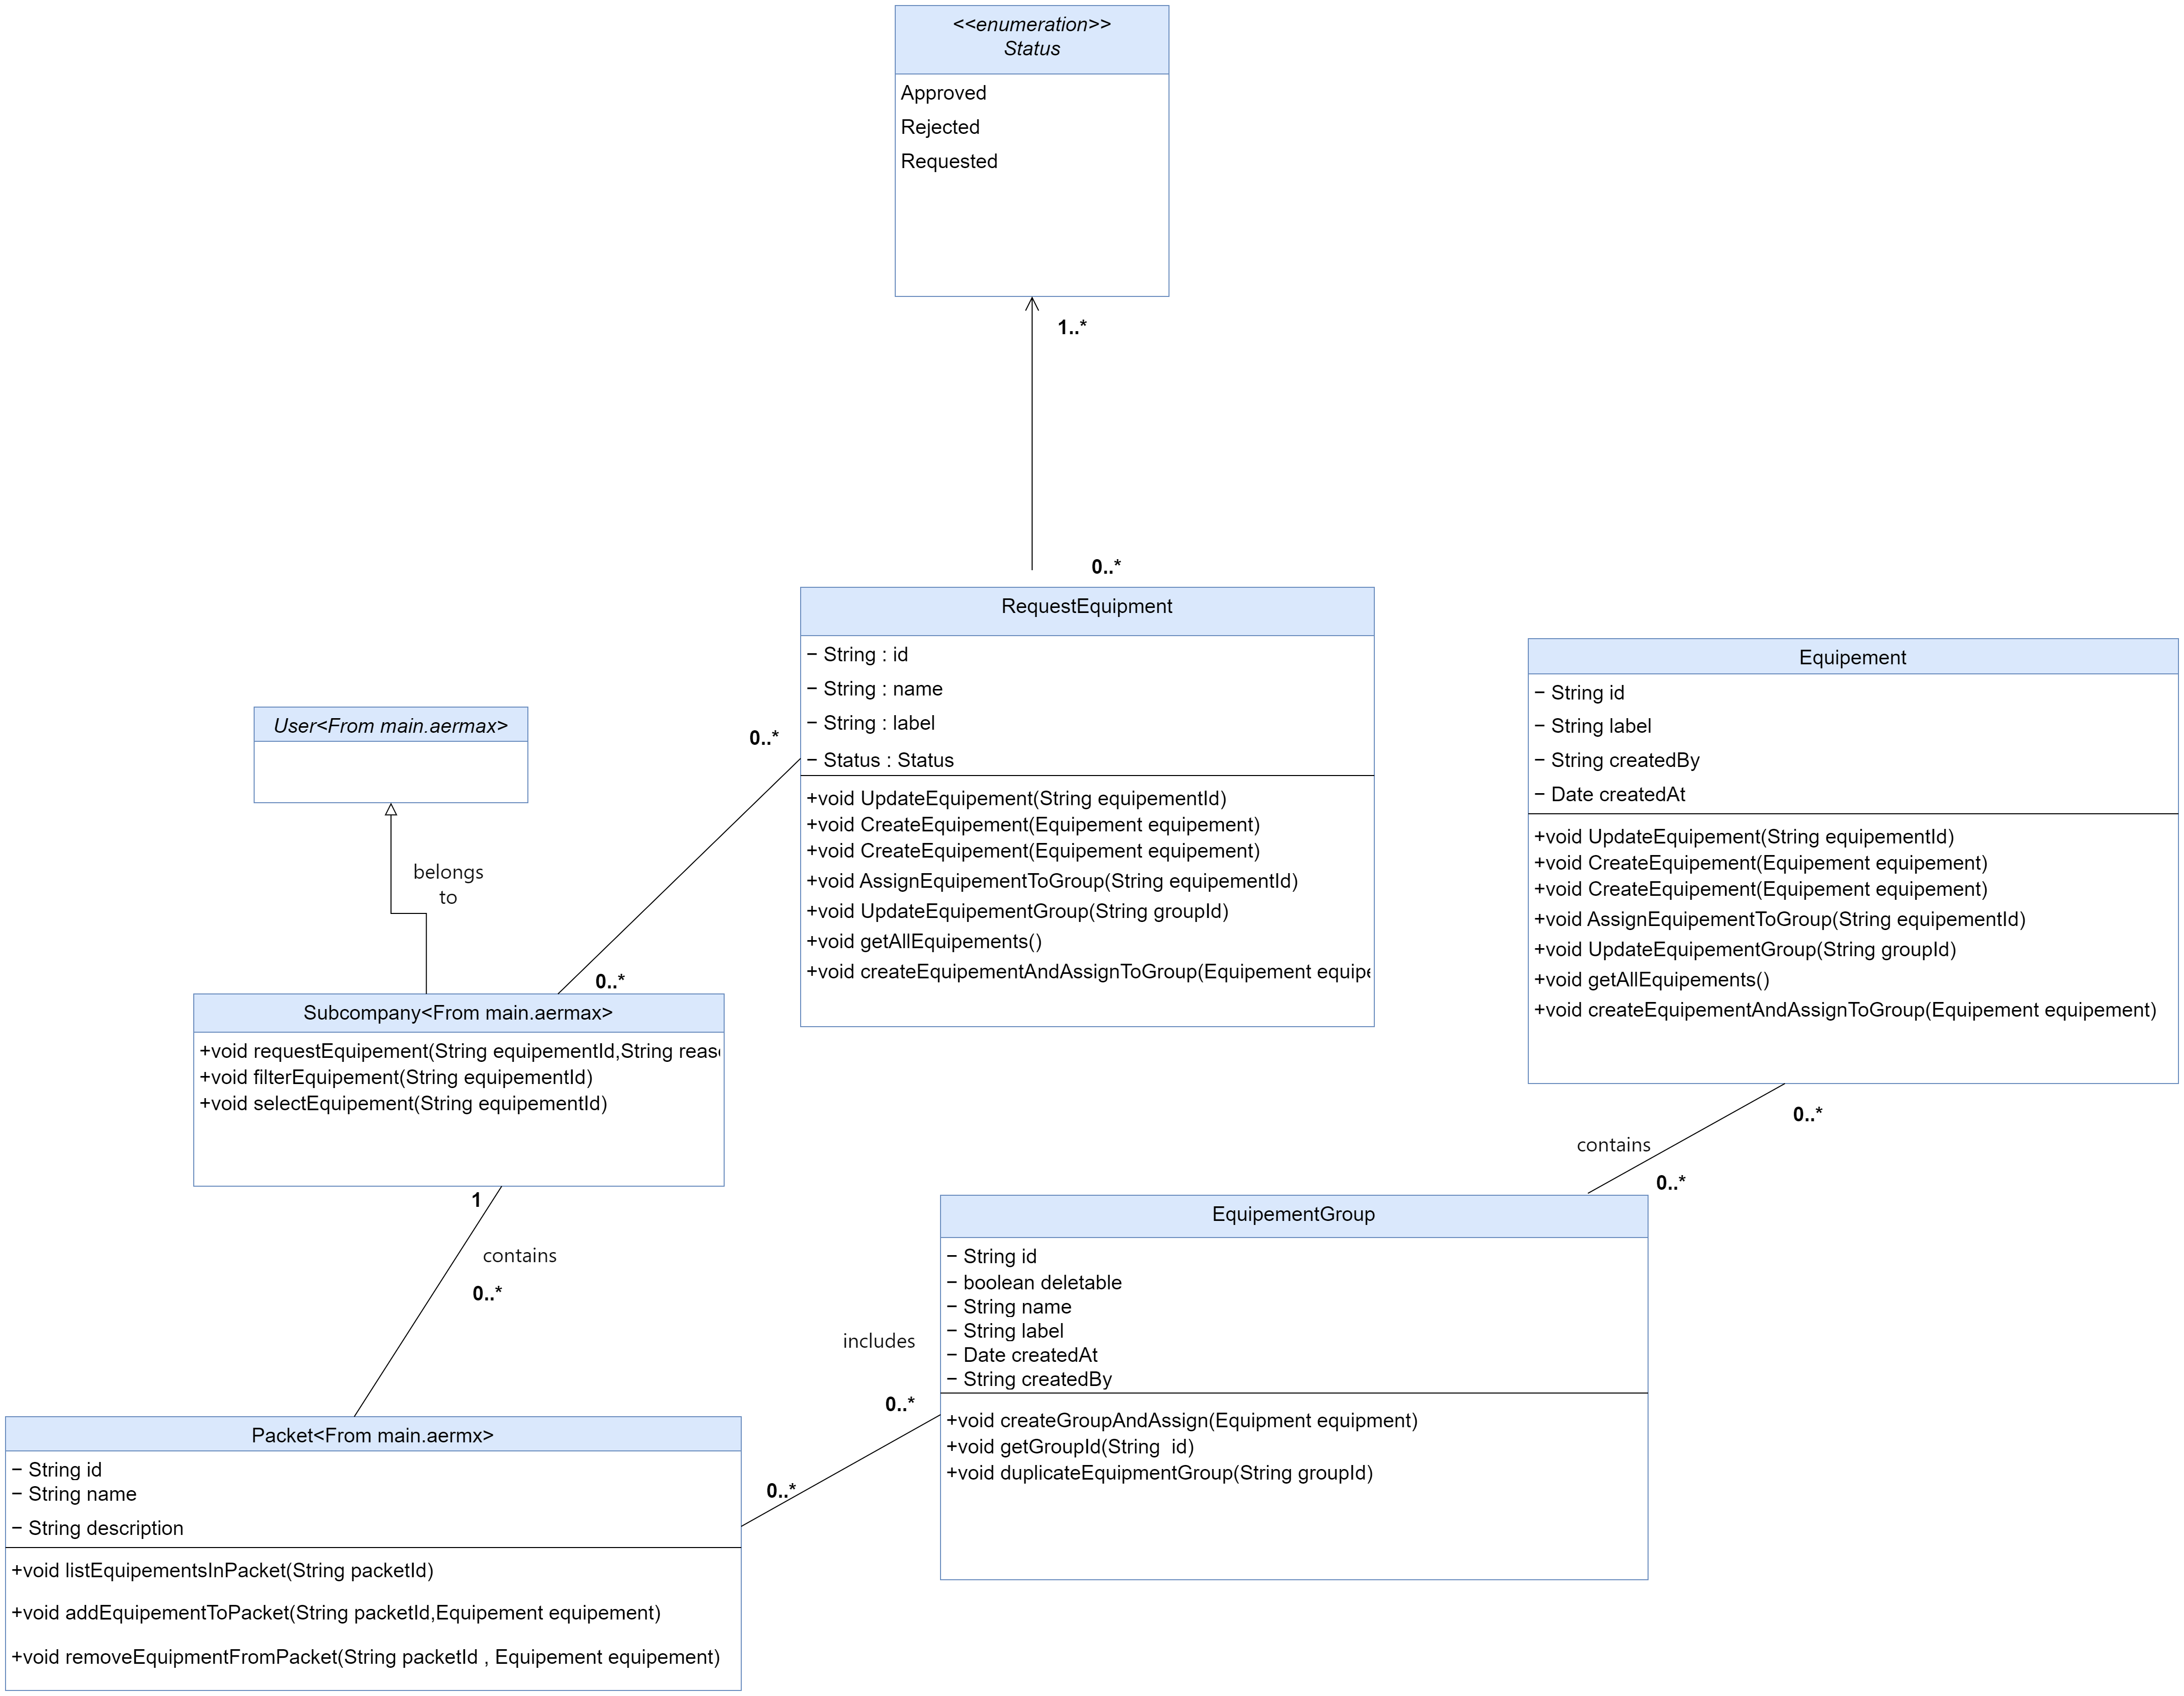
\includegraphics[width=1\textwidth , height=17cm]{src/assets/diagrams/DynamiEquipementListPng.png}
    \caption{Class Diagram for Dynamic Equipment List}
    \label{fig:class_diagram}
\end{figure}
 
\paragraph{Subcompany Interface}
The images below show the subcompany interface after the implementation of the dynamic equipment list, illustrating the improved user experience for subcompany users (see Fig. \ref{fig:subcompany_interface_1}).

\begin{figure}[H]
    \centering
    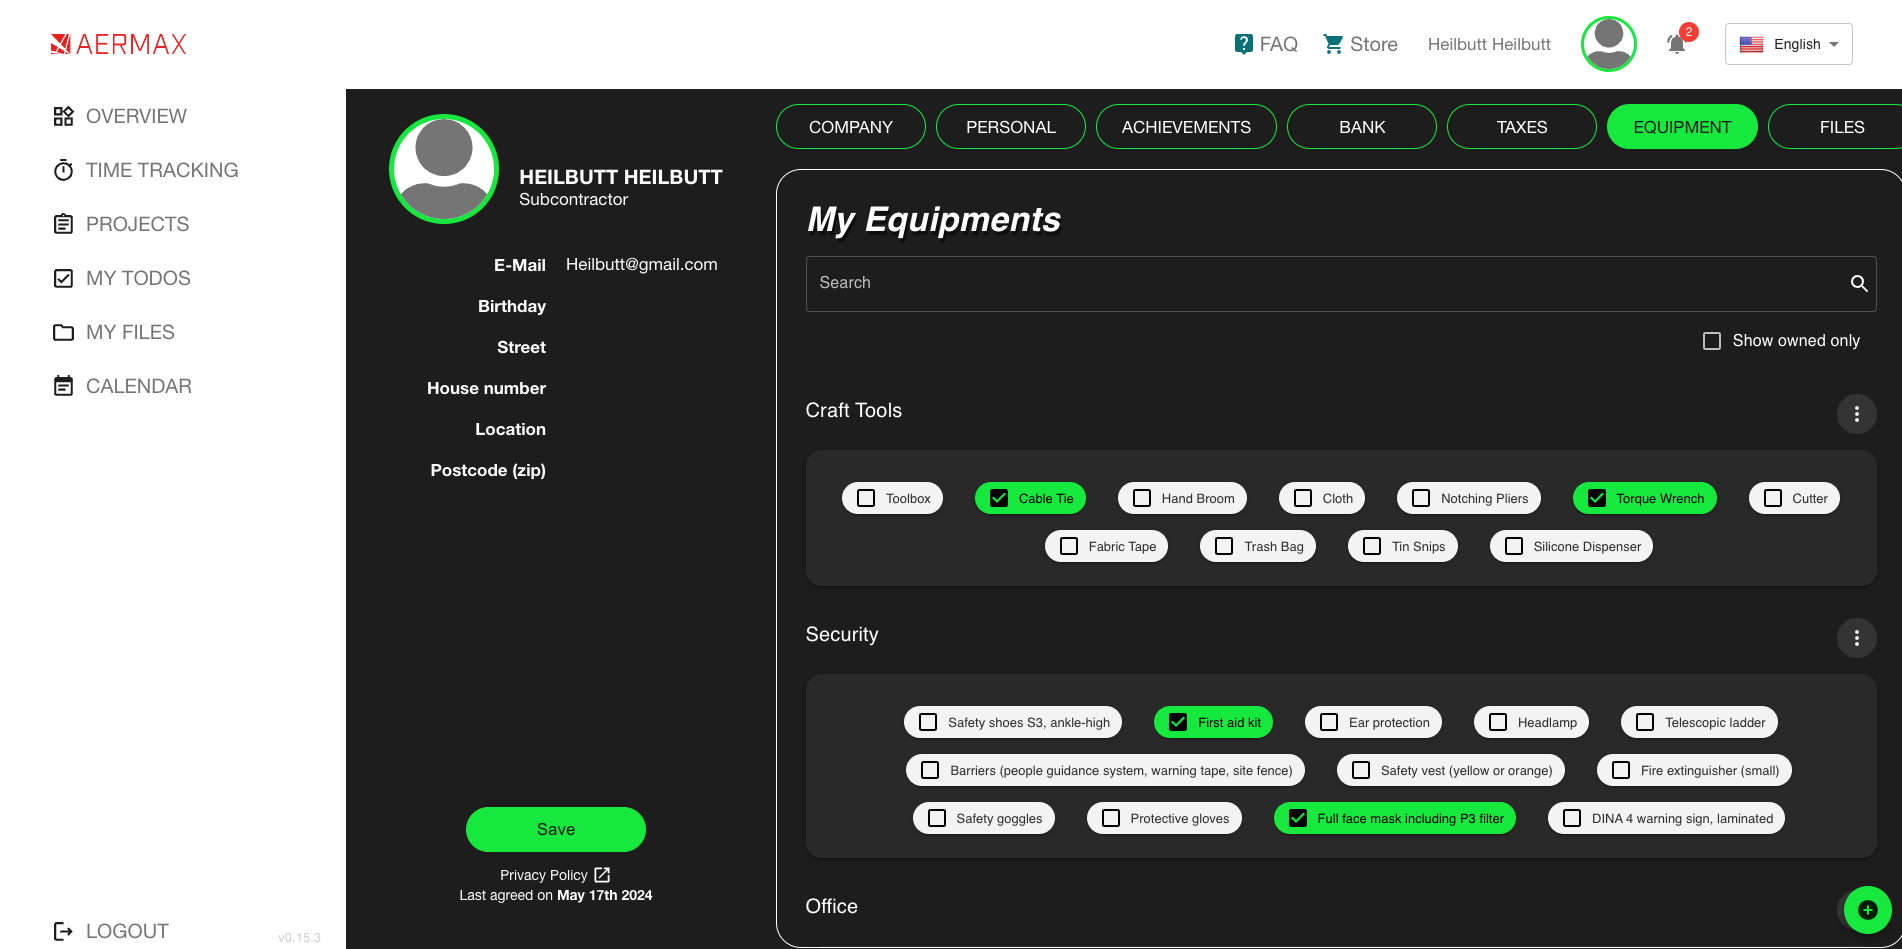
\includegraphics[width=0.9\textwidth]{src/assets/images/Interface1.png}
    \caption{Subcompany Interface - Viewing Assigned Equipment}
    \label{fig:subcompany_interface_1}
\end{figure}

\subsection{Overhaul of the Project Status}

The Aermax platform has undergone a strategic overhaul of the project status functionality to streamline project lifecycle management and improve visibility for all stakeholders. This enhancement was designed to introduce a more dynamic, intuitive, and color-coded status system that aligns with the operational needs and facilitates better decision-making processes.

\subsubsection{Before the Overhaul:}
\begin{itemize}
    \item The status indicators were limited, lacking the granularity required for nuanced project management.
    \item There was no clear distinction between the various stages of a project, from contemplation to completion.
    \item Subcontractors had limited visibility, which sometimes led to inefficiencies and a lack of coordination.
\end{itemize}

\subsubsection{After the Overhaul:}
\begin{itemize}
    \item We've implemented a comprehensive status system, which includes new states such as 'In Progress', 'Closed', 'Re-activated', and 'Cancelled', each represented by distinct color codes.
    \item The status 'In Progress' (green) is particularly significant as it is the only type of project visible to subcontractors, ensuring they have access to relevant, actionable projects.
    \item 'Closed/Finished' projects are denoted with a dark blue color, signifying completion, while 'Re-activated' projects can revert from 'Closed' status when a customer requires additional work or services.
    \item Projects that are no longer active are labeled as 'Cancelled' and are represented in red, providing immediate visual cues for the current state of a project.
    \item A migration process has been instituted to update all existing projects to conform to the new status system, which includes modifying the projectStatus enum to the updated states.
\end{itemize}



\subsubsection*{Technical Enhancements:}
\begin{itemize}
    \item The AggregatedPhase class now includes an attribute that reflects the phase status based on the progress of the included working packets.
    \item The rules for phase status determination are as follows:
        \begin{itemize}
            \item 'Open' by default or when all included packets are open.
            \item 'Completed' if all packets within the phase are completed.
            \item 'Cancelled' if all packets are canceled.
            \item 'In Progress' if there is any packet currently active.
        \end{itemize}
    \item The calendar interface has been upgraded to hide/show project phases and working packets based on their completion or cancellation status, allowing for a cleaner and more focused view.
    \item Events in the calendar have been color-coded to correlate with the status of the project phase or working packet, enhancing the visual experience and making it easier for users to digest the project's progress at a glance.
\end{itemize}

\subsubsection{Visual Enhancement:}
This figure illustrates the enhanced project filter interface, showcasing intuitive filtering options for project number, project status, and state, complete with color-coded status indicators.

\begin{figure}[H]
    \centering
    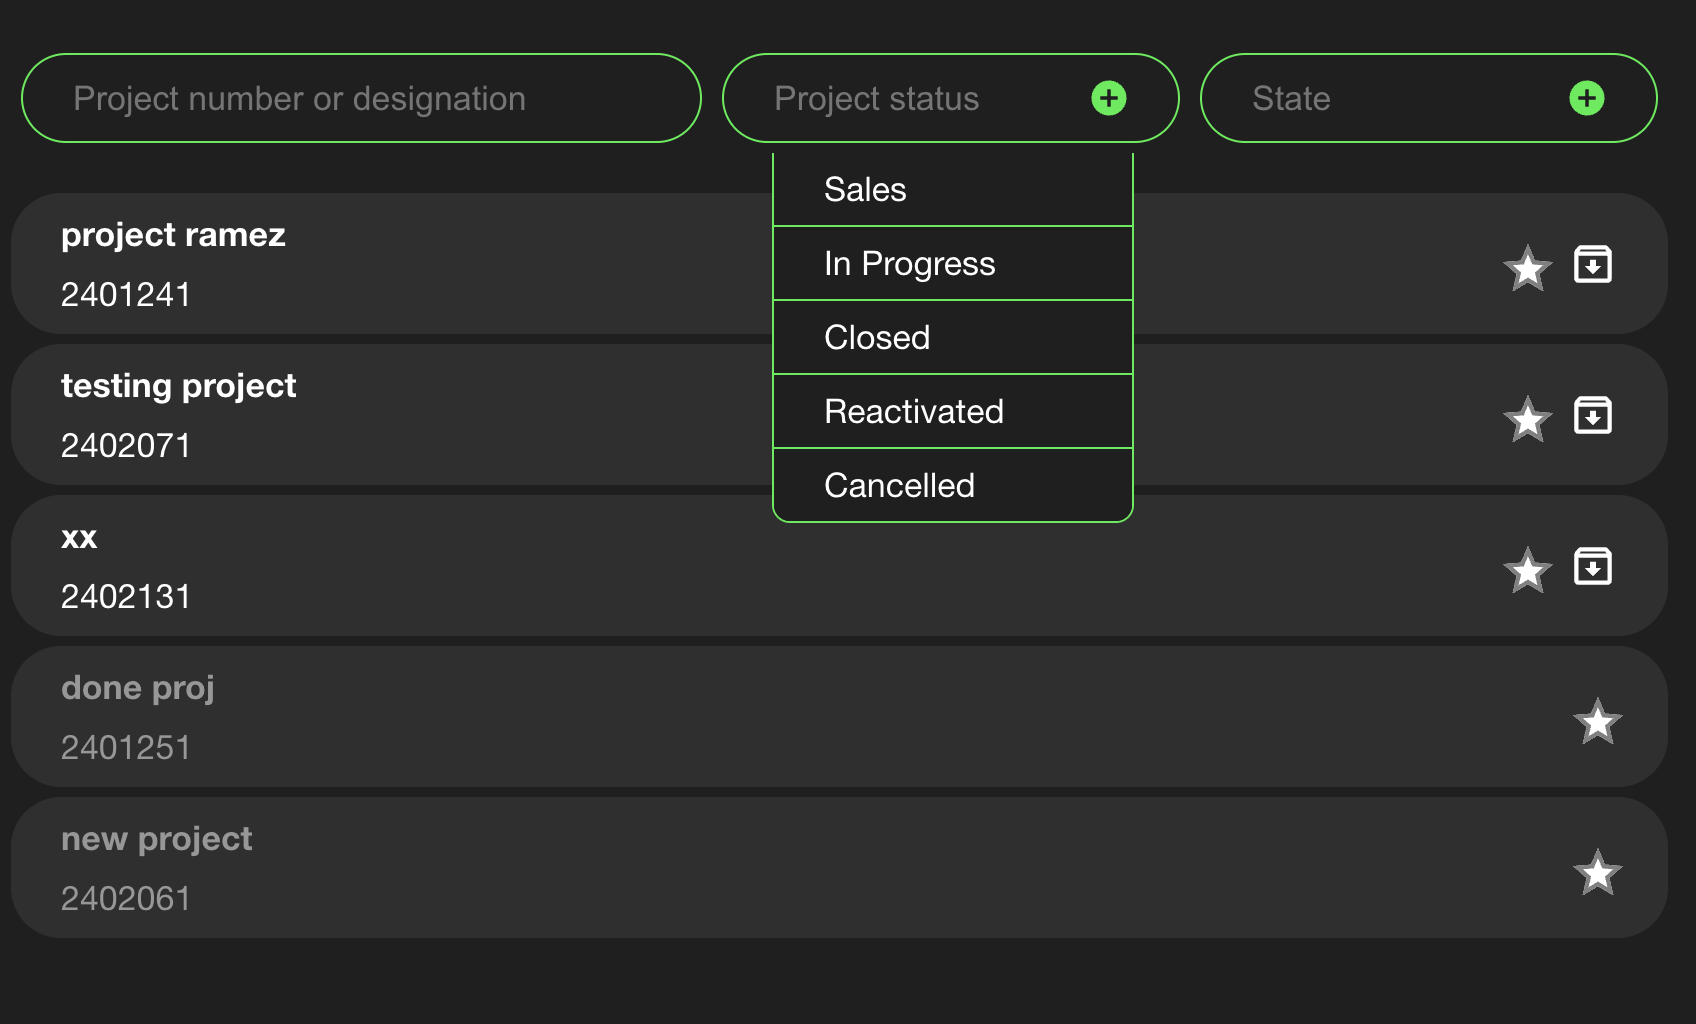
\includegraphics[width=0.9\textwidth]{src/assets/chapters/enhanced-project-filter-interface.png}
    \caption{ Enhanced Project Filter Interface}
    \label{fig:enhanced_project_filter_interface}
\end{figure}

\begin{figure}[H]
    \centering
    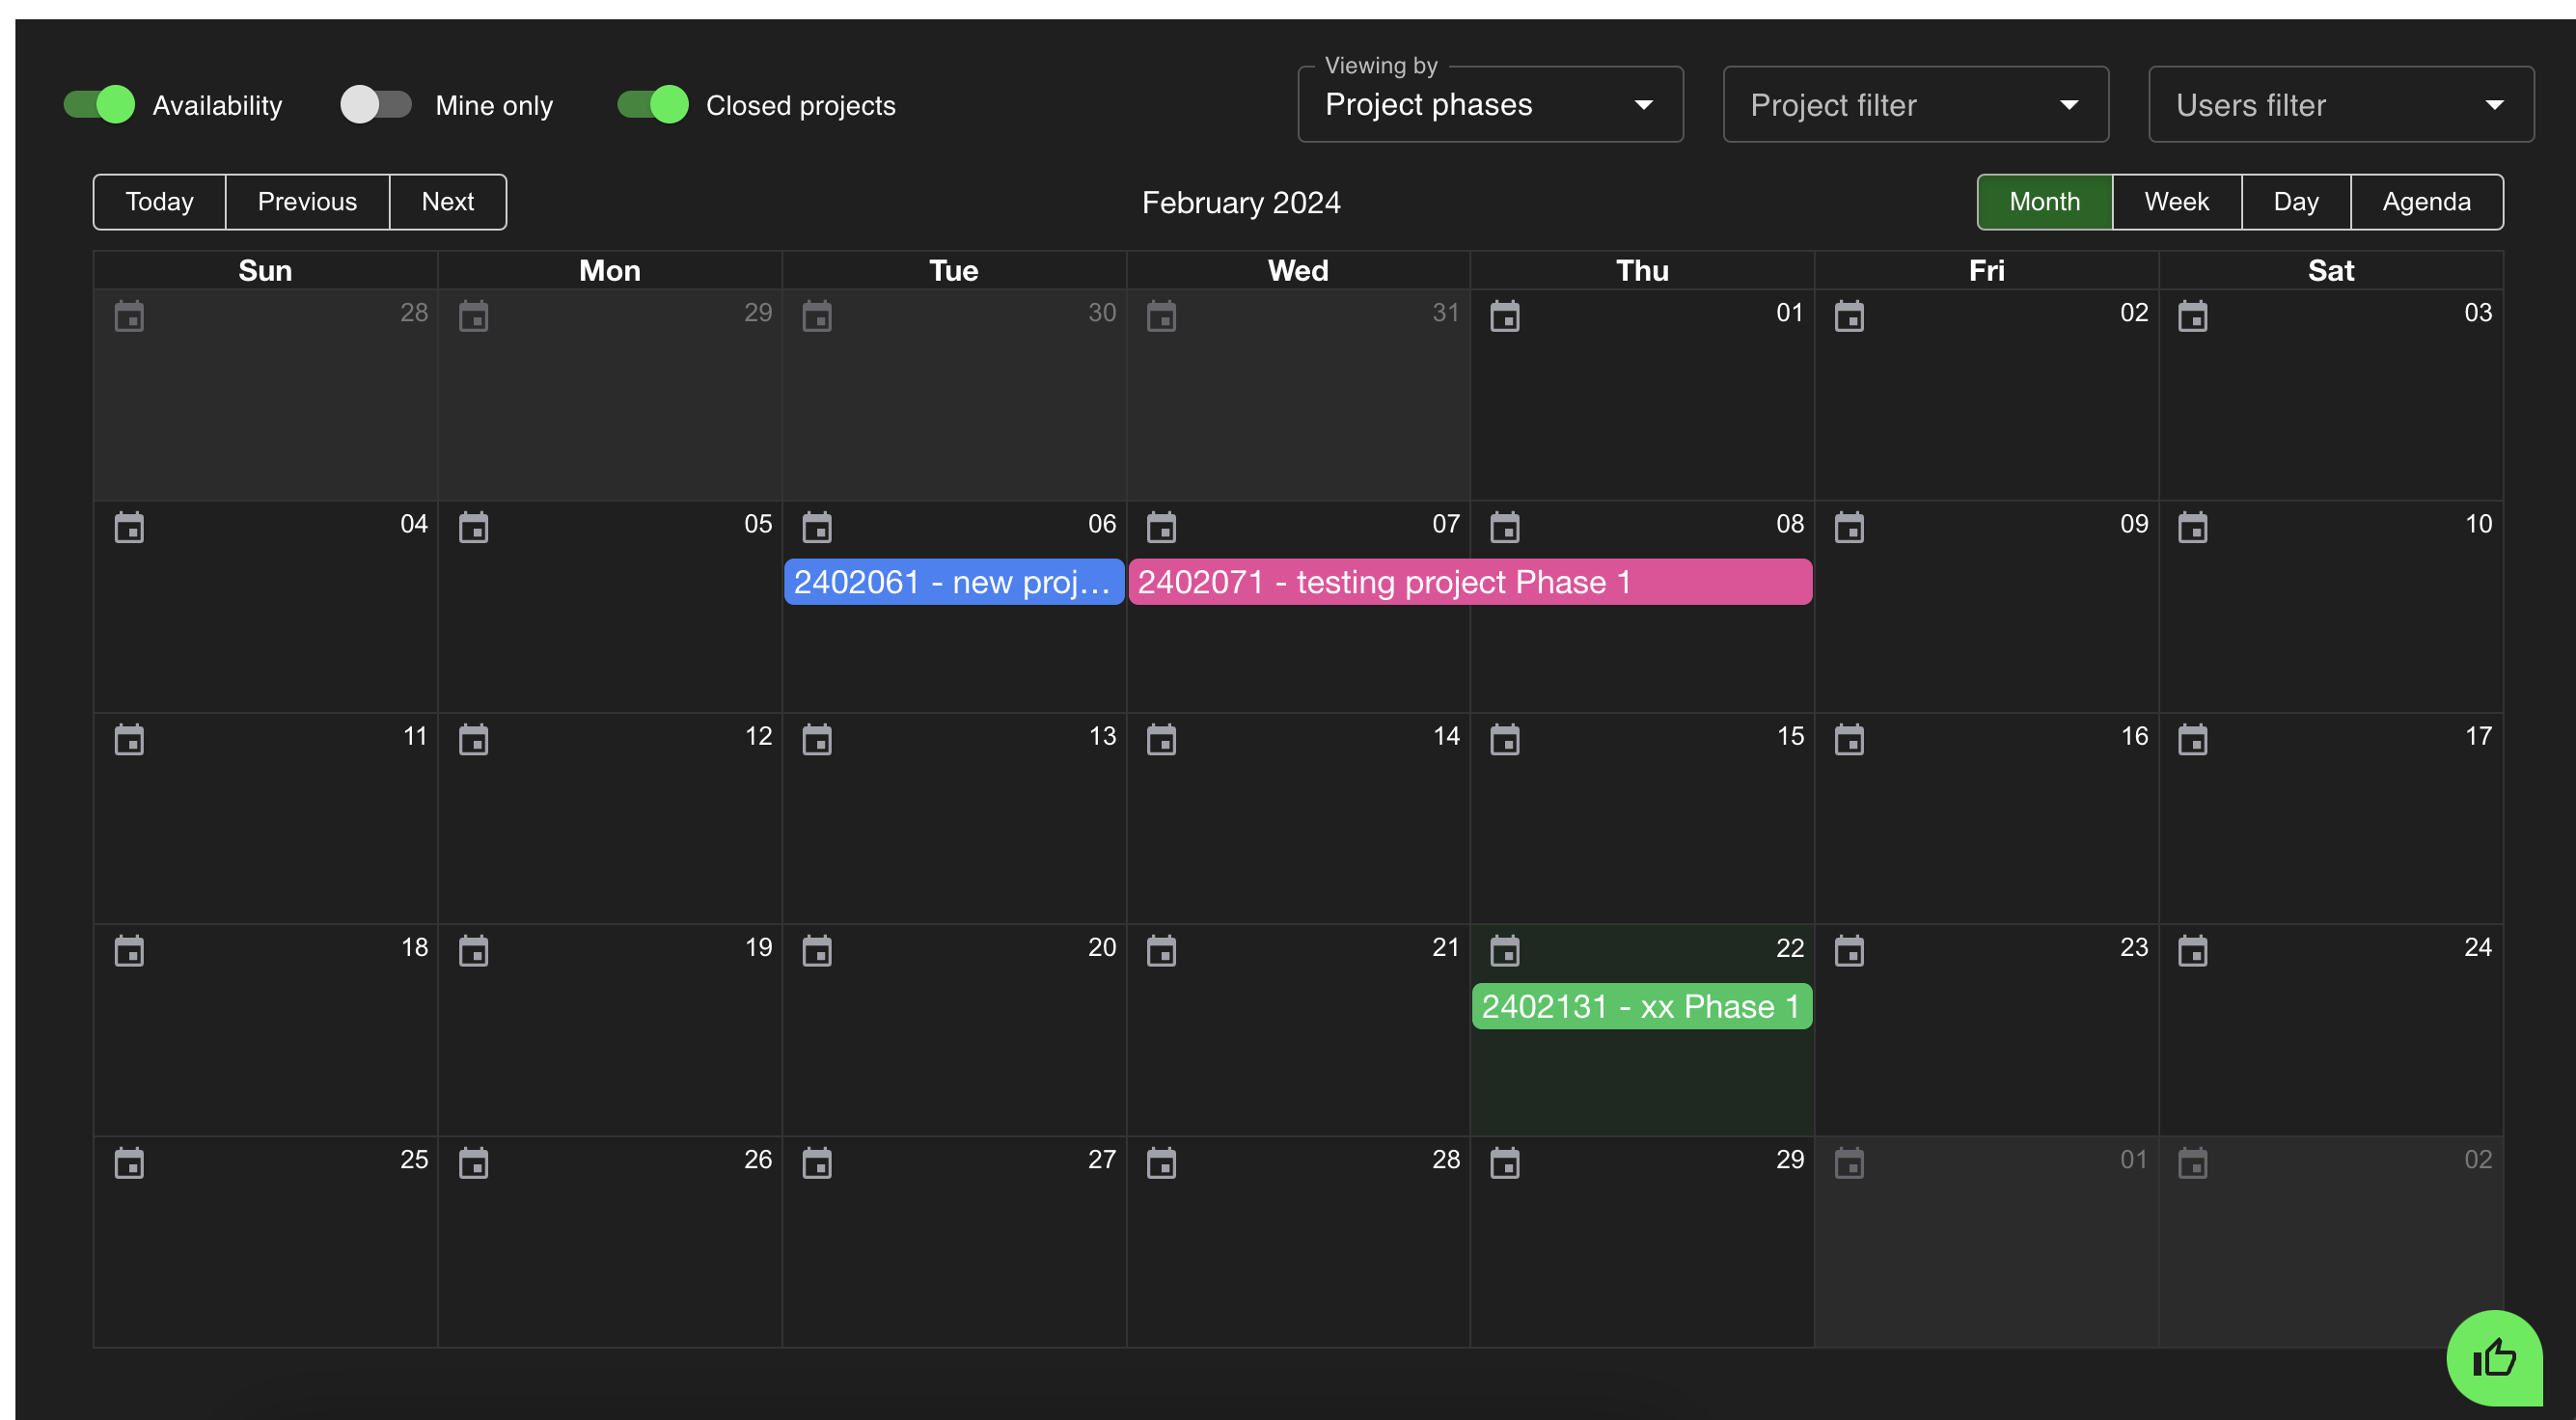
\includegraphics[width=0.9\textwidth]{src/assets/chapters/calendar1.png}
    \caption{Calendar View with Color-Coded Project Phases}
    \label{fig:calendar_view_color_coded}
\end{figure}

\begin{figure}[H]
    \centering
    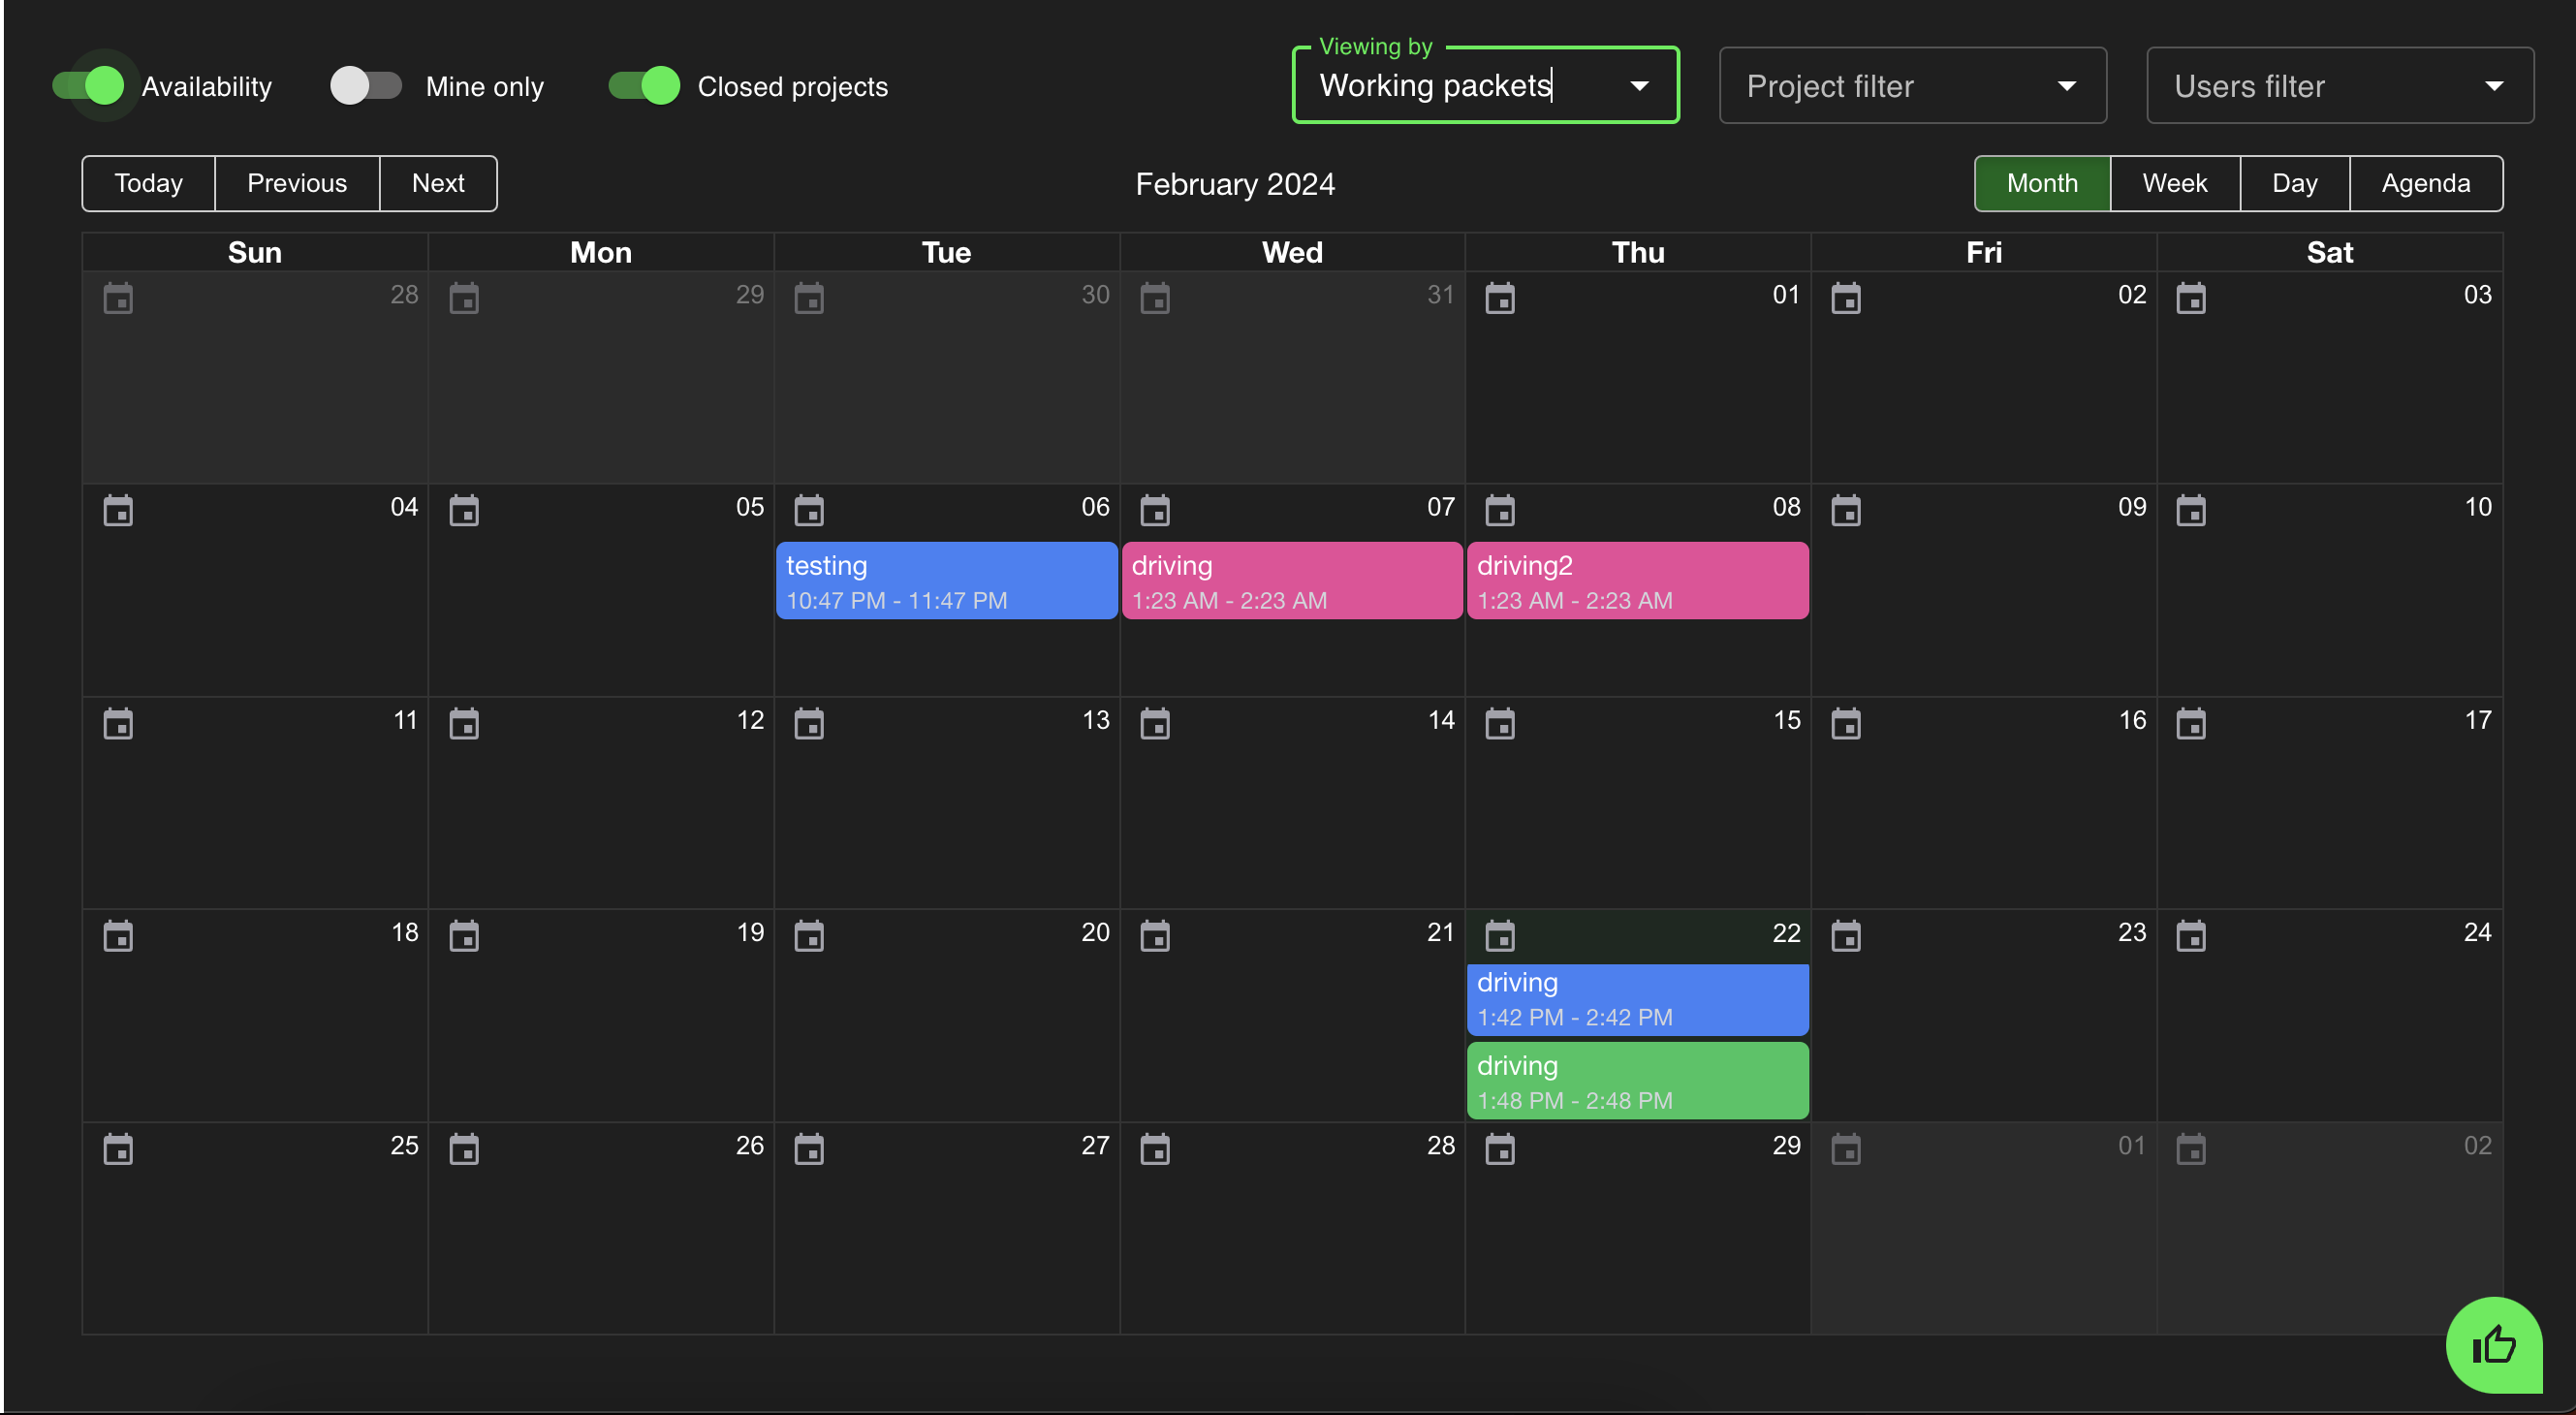
\includegraphics[width=0.9\textwidth]{src/assets/chapters/calendar2.png}
    \caption{Detailed Calendar View of Working Packets with Status Indicators}
    \label{fig:detailed_calendar_view}
\end{figure}



\subsection{Overhaul of the Role System}
Before the Sprint 1 overhaul, the Aermax platform's role system was less delineated, with certain roles having either too broad or too narrow a range of permissions. This occasionally led to confusion, inefficiencies, and security concerns. For instance, Team Leaders had the same project creation rights as Administrators, and Workers had visibility into project overviews that were not relevant to their tasks.

After the Sprint 1 overhaul, we introduced a more refined role system, ensuring that permissions are tightly aligned with the responsibilities intrinsic to each role. The system was restructured to provide a balance between usability and security, reducing the cognitive load on users by limiting their interfaces to the features and information they need for their specific roles.

\subsubsection{Detailed Role Permissions Before \& After}
\begin{longtable}{|p{2.5cm}|p{2cm}|p{2cm}|p{2cm}|p{2cm}|p{2cm}|p{2cm}|p{3cm}|}
\caption{A before-and-after comparison of the detailed role permissions on the Aermax platform.} \label{tab:role_permissions_comparison} \\
\hline
\textbf{Role} & \textbf{View Packets Before} & \textbf{View Packets After} & \textbf{Create Projects Before} & \textbf{Create Projects After} & \textbf{Overview Feature Before} & \textbf{Overview Feature After} & \textbf{Additional Notes (After)} \\ \hline
\endfirsthead

\multicolumn{8}{c}%
{{\bfseries Table \thetable\ Continued from previous page}} \\
\hline
\textbf{Role} & \textbf{View Packets Before} & \textbf{View Packets After} & \textbf{Create Projects Before} & \textbf{Create Projects After} & \textbf{Overview Feature Before} & \textbf{Overview Feature After} & \textbf{Additional Notes (After)} \\ \hline
\endhead

\hline
\multicolumn{8}{|r|}{{Continued on next page}} \\ \hline
\endfoot

\hline
\endlastfoot

Administrator & All & All & Yes & Yes & Yes & Yes & Full system access \\ \hline
Employee & All & All & Yes & Yes & Yes & Yes & Administrative access \\ \hline
Project Manager & All & Specific & Yes & Yes (Start/Stop) & Yes & Yes & Administrative access; manage tasks, discussions, files \\ \hline
Worker & All & Own Only & Yes & No & Yes & No & Confined to personal scope of work \\ \hline
Team Leader & All & Phase Specific & Yes & No & Yes & No & Can view own packets and others within their phase; no project creation \\ \hline

\end{longtable}


% The following text can continue after the table in your LaTeX document.
\textbf{Scenario Demonstrations After Overhaul:}
\begin{itemize}
    \item \textbf{Administrator Scenario:} An Administrator maintains complete control, capable of managing all aspects of the project lifecycle.
    \item \textbf{Employee Scenario:} Employees continue to have similar administrative rights, including full packet visibility and project management capabilities.
    \item \textbf{Project Manager Scenario:} Project Managers are now provided with tailored access, capable of managing specific project packets and workflows.
    \item \textbf{Worker Scenario:} Workers are limited to their own packets, focusing their dashboard on personal tasks without additional project creation or overview privileges.
    \item \textbf{Team Leader Scenario:} Team Leaders have targeted oversight, managing only the packets within their project phase, without the distraction of other project overviews or creation capabilities.
\end{itemize}

This targeted approach in the role system refines the user experience on the Aermax platform, ensuring each role has the access needed to perform effectively, securely, and efficiently.

\subsection{Enhance Working Packets UI \& UX}
In our continuous efforts to elevate the user experience on the Aermax platform, a significant upgrade was made to the Working Packets UI \& UX, particularly focusing on the administrative interface. 

\begin{figure}[H]
    \centering
    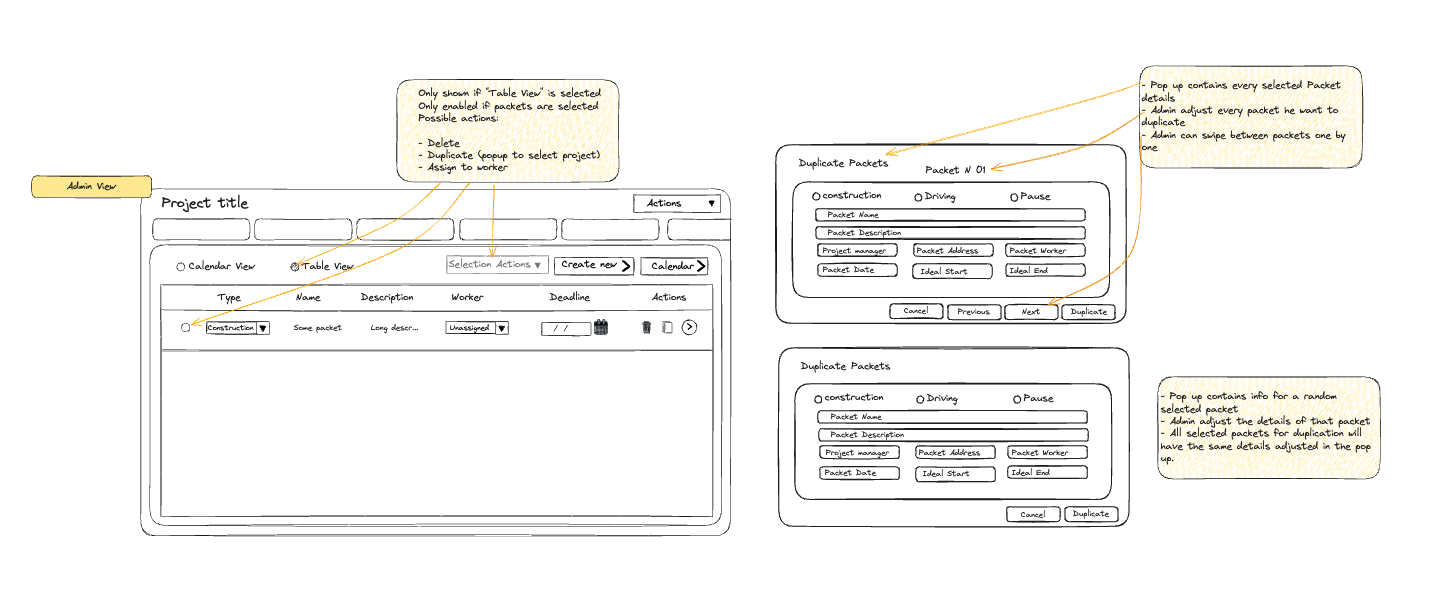
\includegraphics[width=1.1\textwidth]{src/assets/chapters/ui_ux-enhancement.png}
    \caption{Sketch of Planned UI/UX Enhancements for Working Packets }
    \label{fig:ui_ux_enhancements}
\end{figure}


\begin{figure}[H]
    \centering
    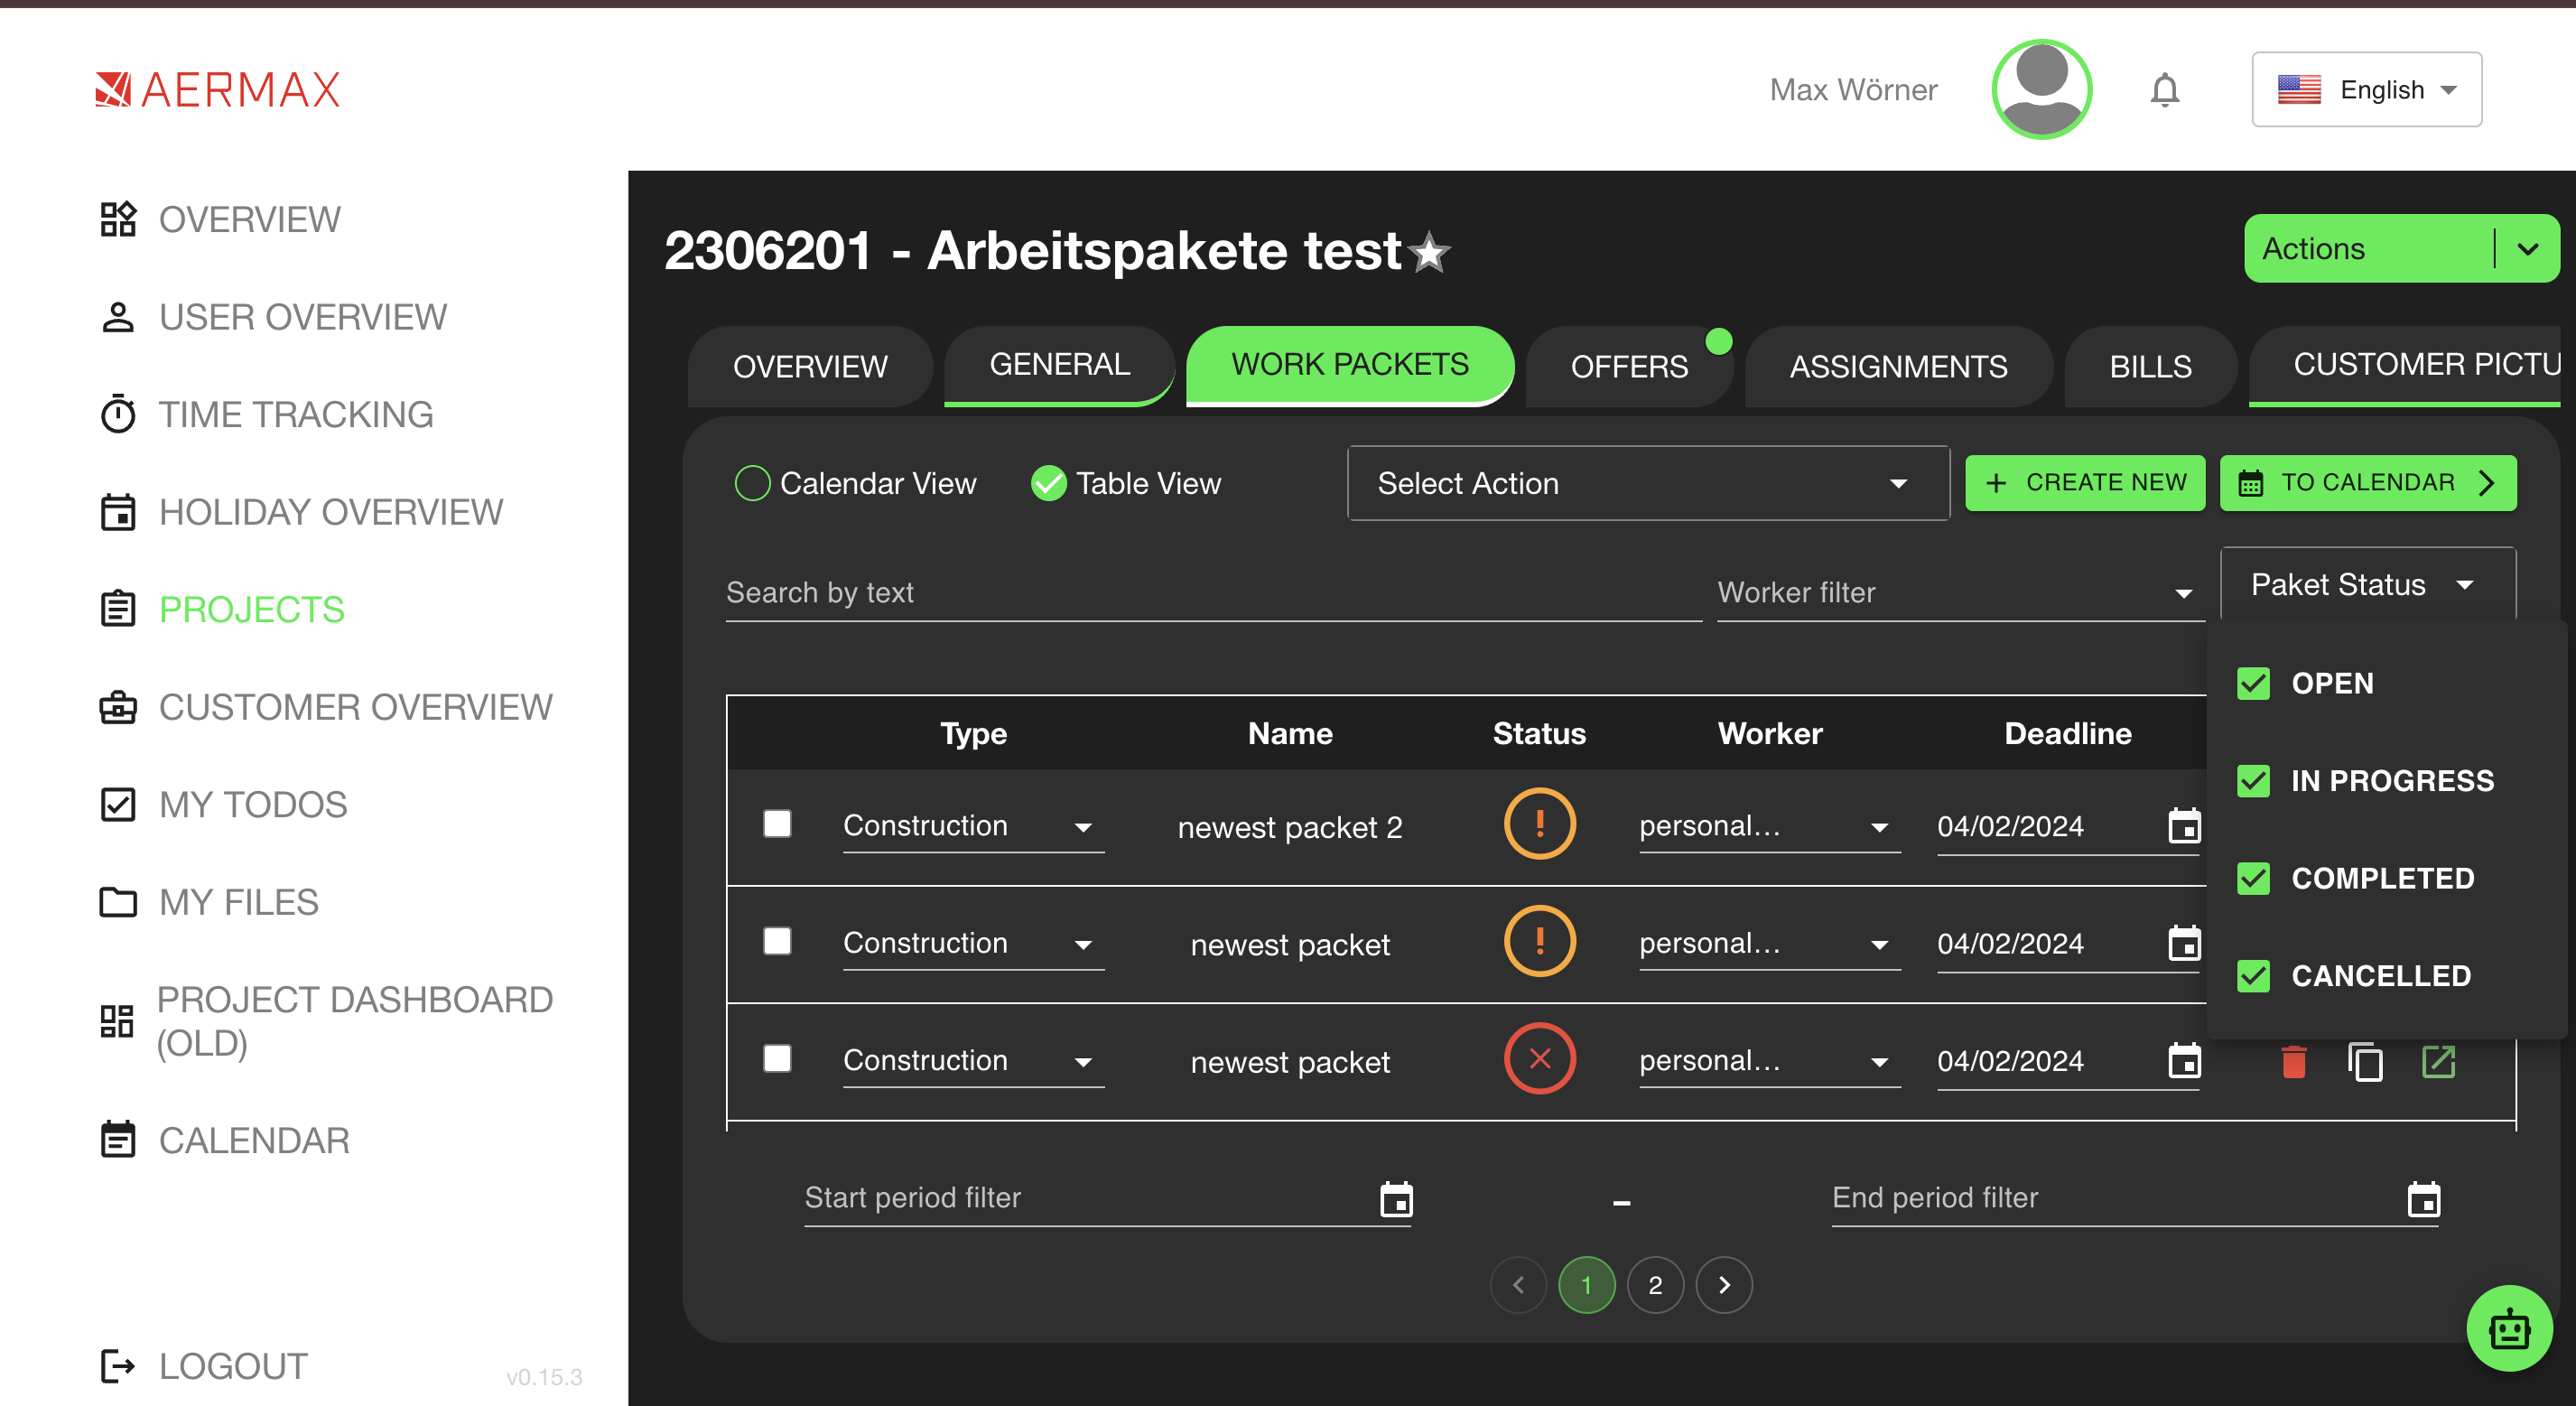
\includegraphics[width=0.9\textwidth]{src/assets/chapters/newTable1.png}
    \caption{Sketch of Planned UI/UX Enhancements for Working Packets }
    \label{fig:ui_ux_enhancements}
\end{figure}


\begin{figure}[H]
    \centering
    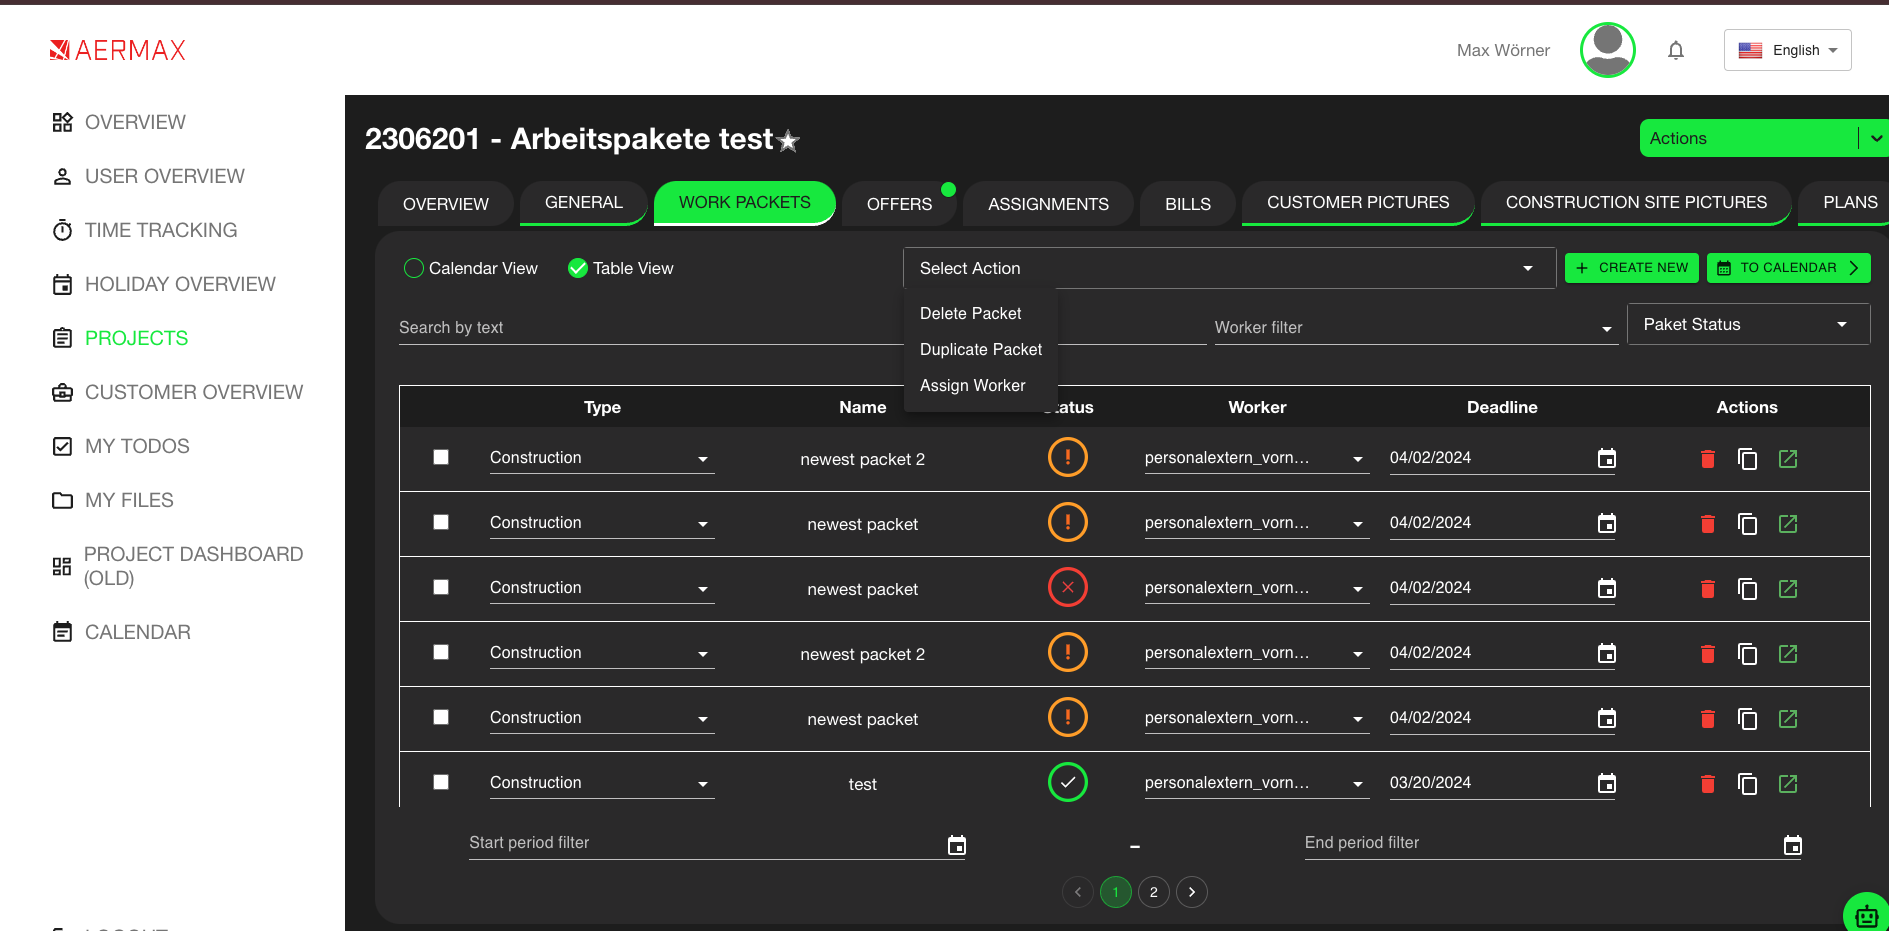
\includegraphics[width=0.9\textwidth]{src/assets/chapters/newTable2.png}
    \caption{Sketch of Planned UI/UX Enhancements for Working Packets }
    \label{fig:ui_ux_enhancements}
\end{figure}

\subsection{Self Registration}

We have implemented a self-registration feature that streamlines the process of user registration, allowing new users to create accounts autonomously.

\begin{figure}[H]
    \centering
    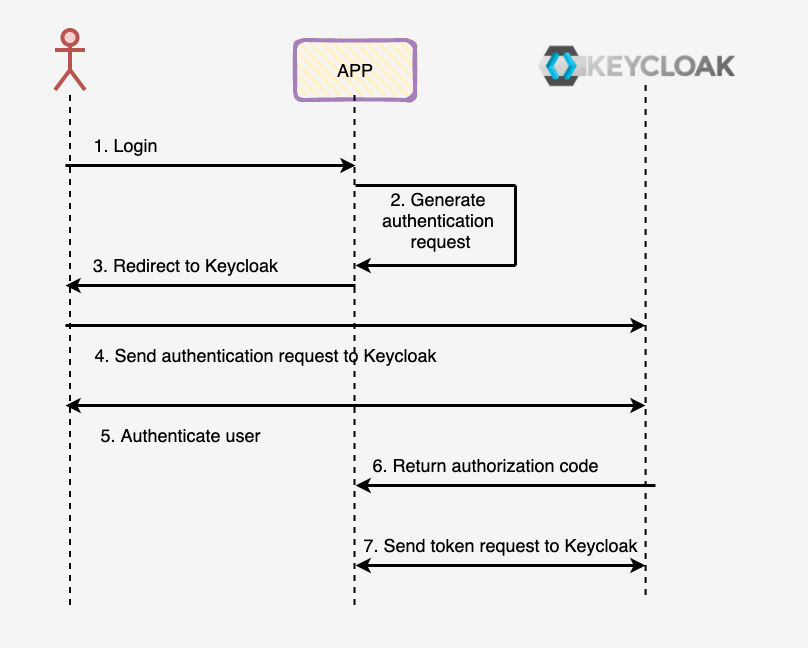
\includegraphics[width=0.9\textwidth]{src/assets/chapters/keycloak-diagram.png}
    \caption{Authentication Flow Using Keycloak: A visual guide to the user authentication process with Keycloak.}
    \label{fig:authentication_flow_keycloak}
\end{figure}

Figure \ref{fig:authentication_flow_keycloak} illustrates the authentication flow using Keycloak. The figure will show the step-by-step authentication flow, demonstrating how users interact with Keycloak during the login process. It provides a visual explanation of the authentication steps from the user initiating a login request to receiving a token from Keycloak.

As part of this overhaul, we encountered the challenge of duplicate user entries due to previous system design limitations. By leveraging Keycloak’s versatile user federation and identity provider features, we were able to consolidate user accounts and eliminate redundancies, thereby solving the issue of duplicate entries. 

Keycloakify complemented this integration by allowing us to customize the authentication pages to align with our platform's aesthetics and usability standards.

\subsubsection{Feature Implementation Table:}
\begin{table}[H]
\centering
\begin{tabularx}{\textwidth}{|X|X|X|}
\hline
\textbf{Feature} & \textbf{Technology Implemented} & \textbf{Description} \\
\hline
Login/Signup & Keycloak, Keycloakify & Integrated with Keycloak to secure and streamline user access, enhanced by Keycloakify for customized UI/UX. \\
\hline
Password Management & Keycloak & Developed a secure and user-friendly password management system, providing users with ease of control over their credentials. \\
\hline
\end{tabularx}
\caption{Summary of Keycloak feature implementations.}
\label{tab:keycloak_features}
\end{table}

\subsection{Backend Enhancements and Data Integrity}
\textbf{Eliminating Duplicate Users and Improving Data Handling}
Our backend team undertook the critical task of enhancing the database and data processing layers of our system. The focus was on refining our data model to eliminate the occurrence of duplicate user entries—a problem that stemmed from a legacy design.
 
\begin{figure}[H]
    \centering
    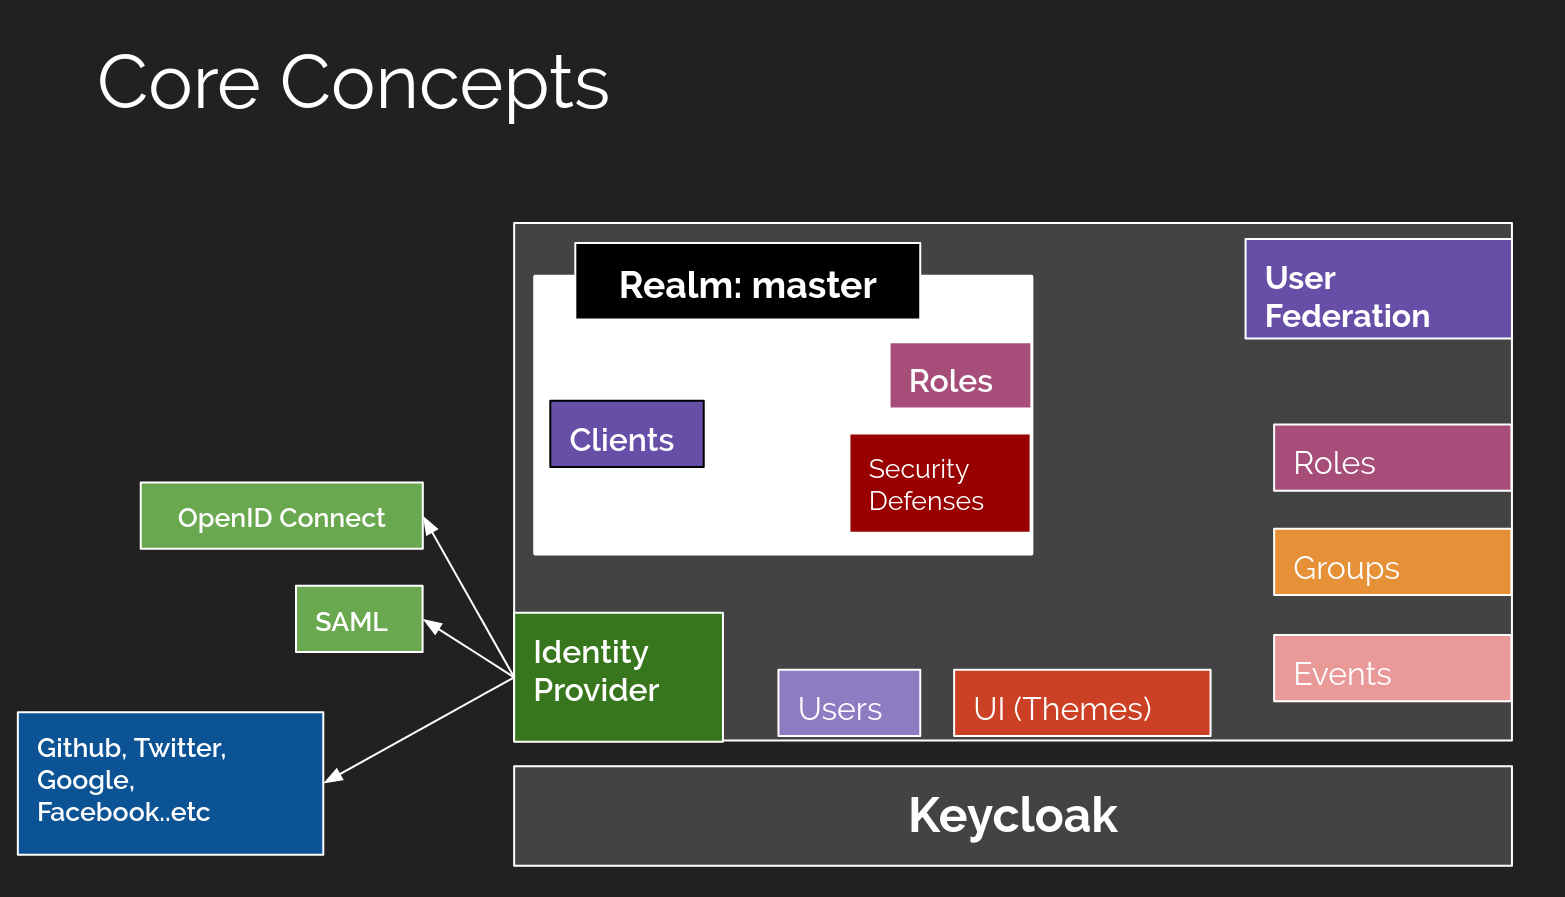
\includegraphics[width=0.9\textwidth]{src/assets/chapters/core-conccept.png}
    \caption{Core Concepts of Keycloak's Architecture}
    \label{fig:core_concepts_keycloak}
\end{figure}

This image will give an overview of Keycloak’s core concepts, such as realms, roles, and identity providers. It visually communicates the architecture that supports the functionality we harnessed to solve our data integrity challenges.


\subsection{UI/UX Design Improvements}
\addcontentsline{toc}{subsection}{UI/UX Design Improvements}
With user experience at the forefront of our digital solution, the Aermax platform underwent a significant UI/UX redesign to enhance cleanliness, intuitiveness, and functionality. Using Figma, our design team was able to collaborate on and iterate high-fidelity mockups and prototypes, which provided a visual roadmap for the platform's evolution.

\textbf{Objective:} To revamp the Aermax platform's design for a more streamlined, user-friendly interface that aligns with modern standards and enhances user engagement.

\textbf{Outcome:} The design overhaul has resulted in a cleaner and more intuitive interface that simplifies user interactions and reduces cognitive load. With a focus on ease of use, the new design has improved the overall user experience, leading to increased user satisfaction and platform adoption.

\textbf{Visual Demonstration:} The following images compare the original and the new Figma-enhanced UI/UX designs, showcasing the transformation and the design team's dedication to creating a user-centred interface.

 

\begin{figure}[H]
    \centering
    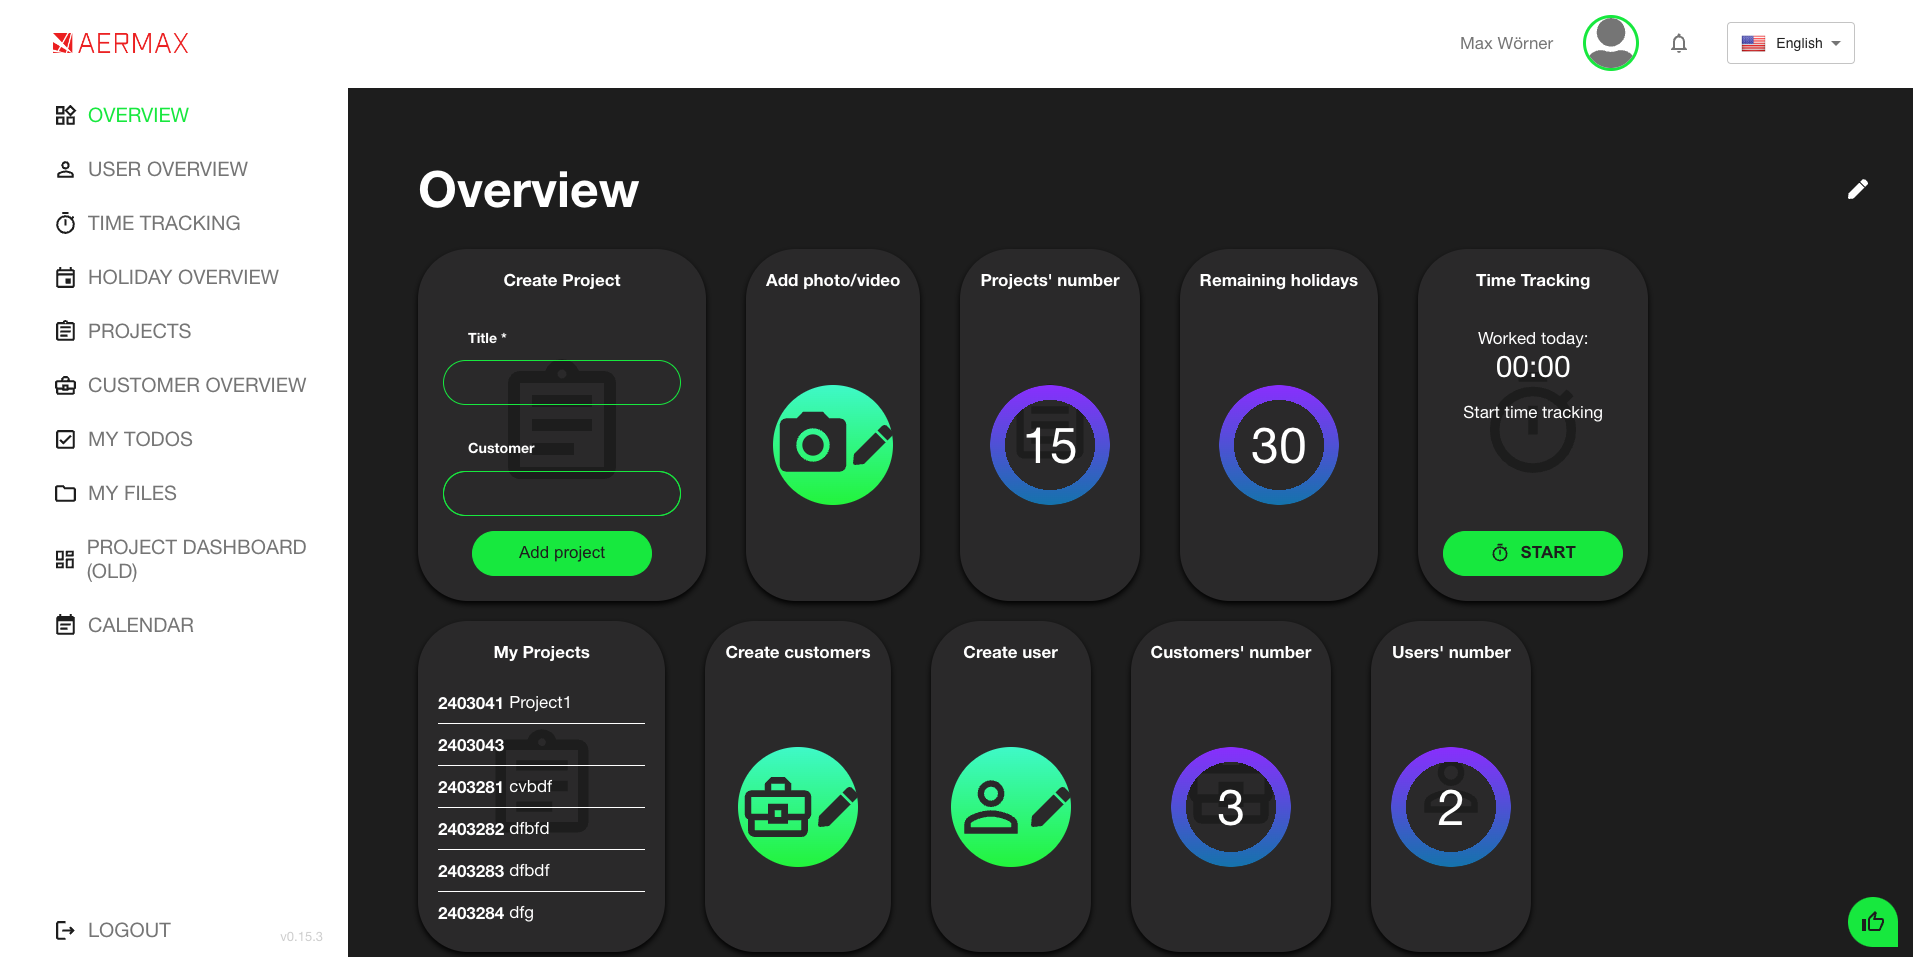
\includegraphics[width=0.9\textwidth]{src/assets/chapters/OverviewPage.png}
    \caption{Original Aermax platform Overview page UI design.}
    \label{fig:overview_page_design}
\end{figure}

\begin{figure}[H]
    \centering
    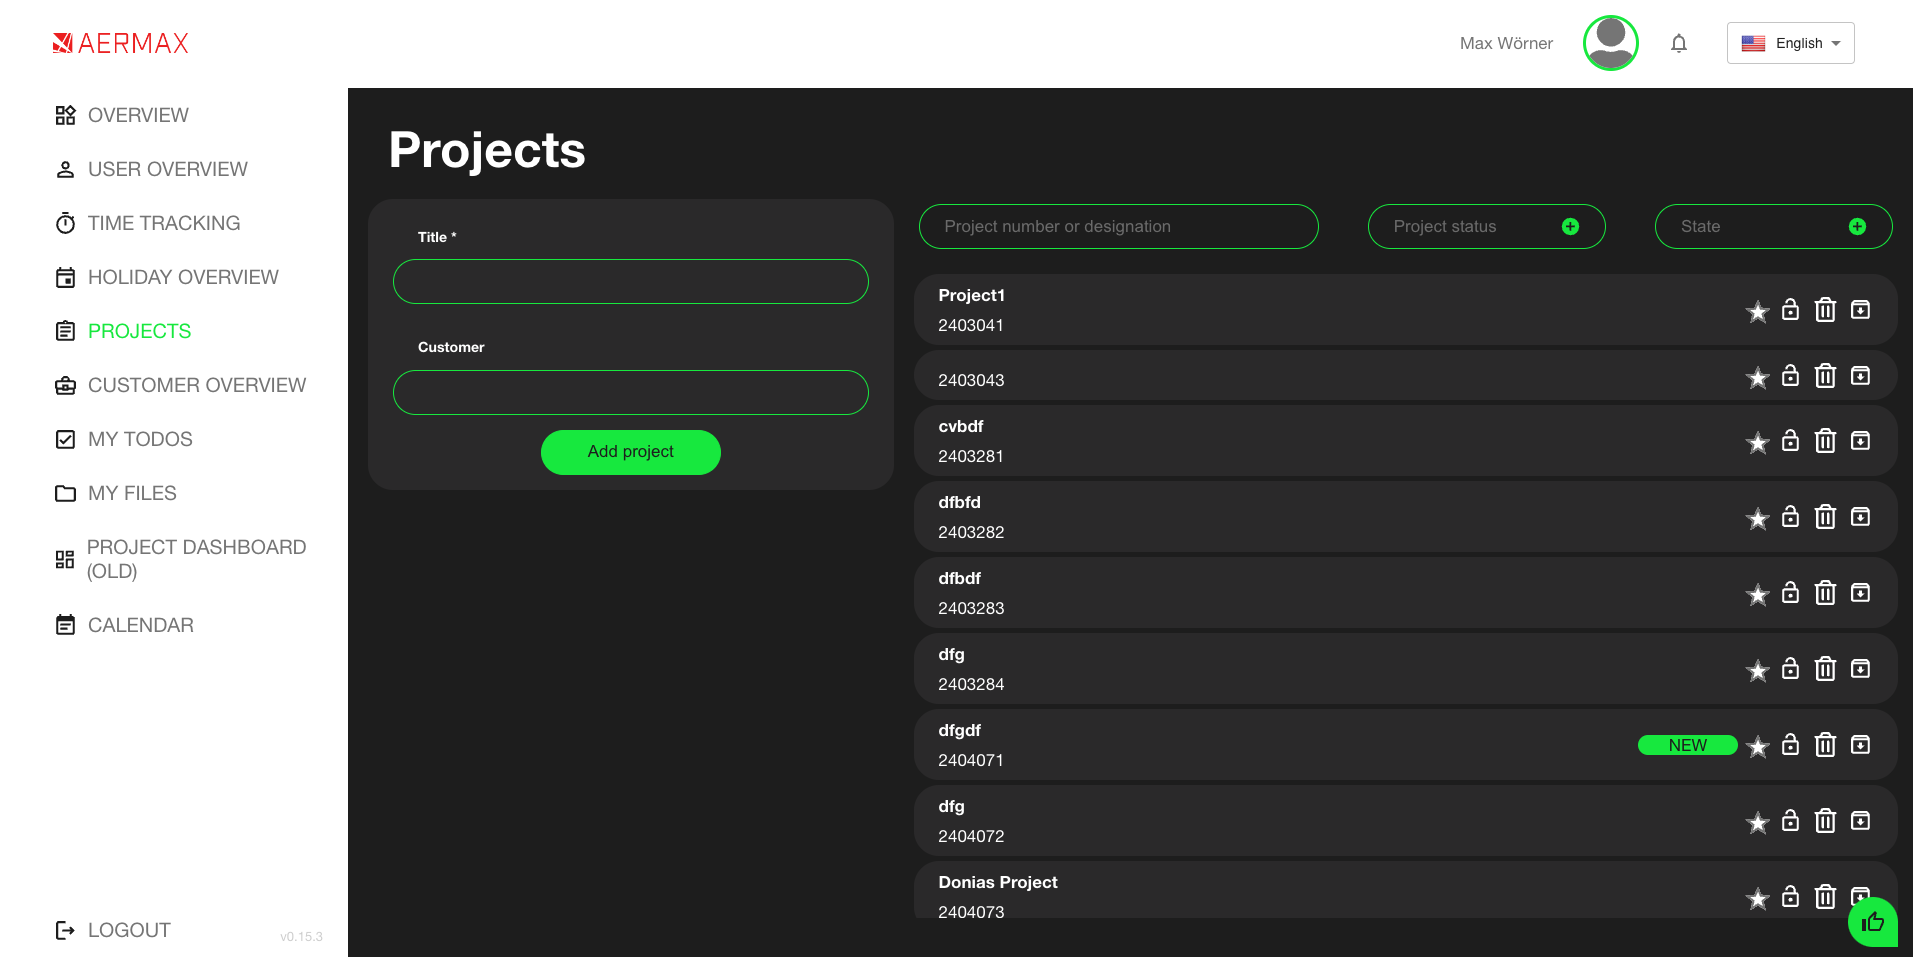
\includegraphics[width=0.9\textwidth]{src/assets/chapters/ProjectPage.png}
    \caption{Original Aermax platform Project page UI design.}
    \label{fig:project_page_design}
\end{figure}


\begin{figure}[H]
    \centering
    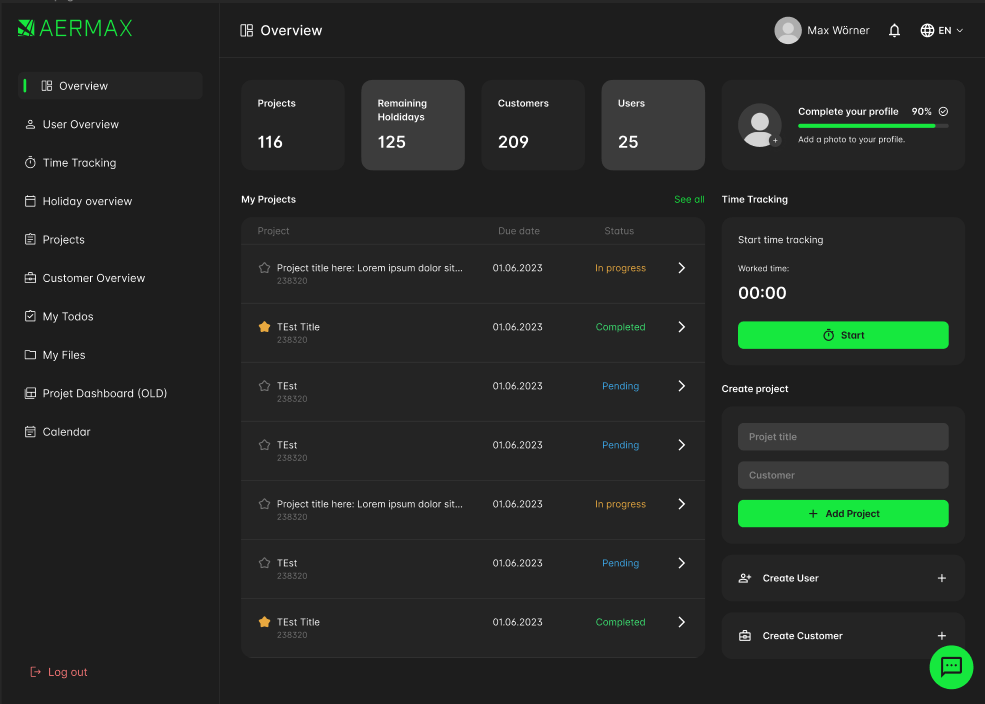
\includegraphics[width=0.9\textwidth]{src/assets/chapters/ui-ux-dashboard.png}
    \caption{Enhanced Aermax platform Overview page UI design in dark mode.}
    \label{fig:enhanced_overview_dark}
\end{figure}

\begin{figure}[H]
    \centering
    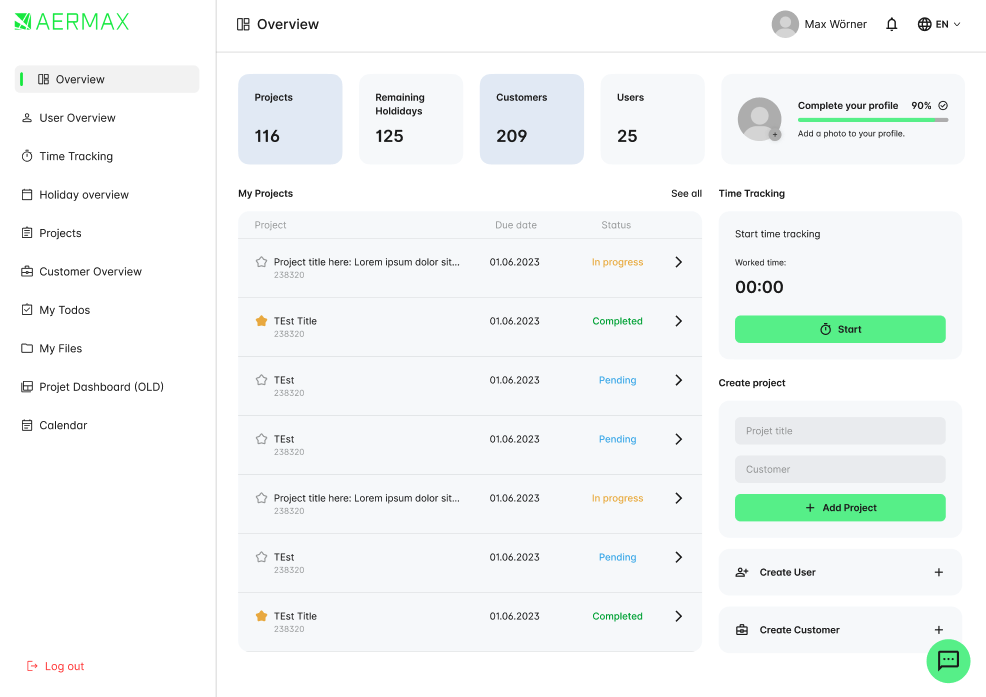
\includegraphics[width=0.9\textwidth]{src/assets/chapters/ui--ux-dashboard.png}
    \caption{Enhanced Aermax platform Overview page UI design in light mode.}
    \label{fig:enhanced_overview_light}
\end{figure}

\begin{figure}[H]
    \centering
    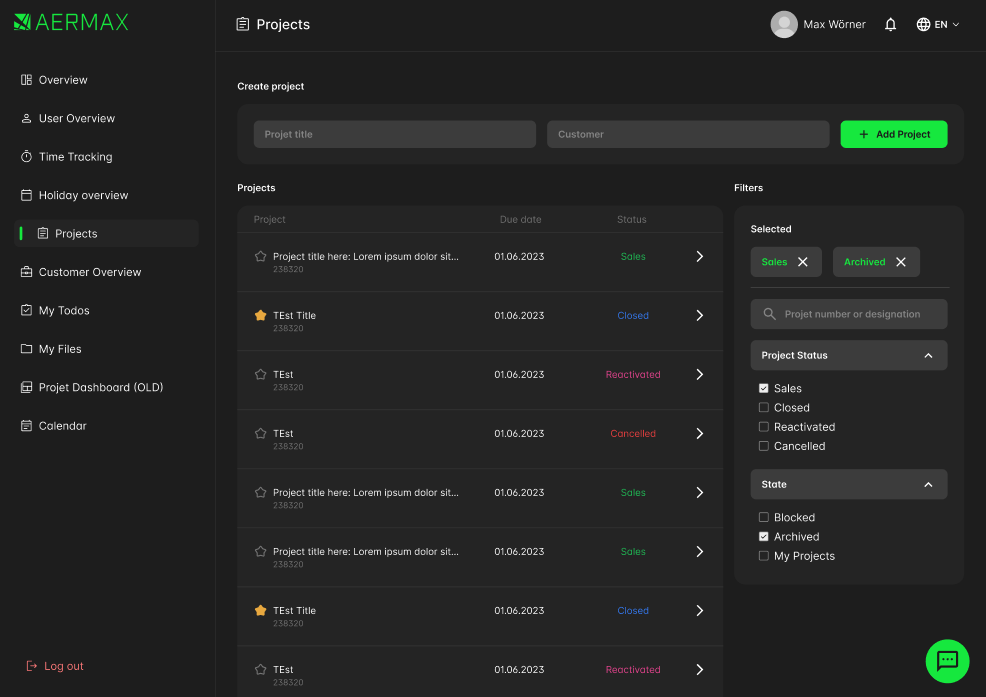
\includegraphics[width=0.9\textwidth]{src/assets/chapters/ui-ux--peoject.png}
    \caption{Enhanced Aermax platform Project page UI design.}
    \label{fig:enhanced_project_page}
\end{figure}

